%%%%%%%% ICML 2023 EXAMPLE LATEX SUBMISSION FILE %%%%%%%%%%%%%%%%%

\documentclass{article}

% Recommended, but optional, packages for figures and better typesetting:
\usepackage{microtype}
\usepackage{graphicx}
% \usepackage{subfigure}
\usepackage{booktabs} % for professional tables
\usepackage{multirow}

% hyperref makes hyperlinks in the resulting PDF.
% If your build breaks (sometimes temporarily if a hyperlink spans a page)
% please comment out the following usepackage line and replace
% \usepackage{icml2023} with \usepackage[nohyperref]{icml2023} above.
\usepackage{hyperref}

% Plots
% \usepackage{tikz}
% \usepackage{pgfplots}
% \pgfplotsset{compat=1.15}
% \usepgfplotslibrary{fillbetween}
% \usetikzlibrary{external}
\usepackage{tikz}
\usepackage{pgfplots}
\pgfplotsset{compat=1.18}
\usepgfplotslibrary{fillbetween}
\usepackage{subcaption}


% Attempt to make hyperref and algorithmic work together better:
\newcommand{\theHalgorithm}{\arabic{algorithm}}

% Use the following line for the initial blind version submitted for review:
% \usepackage{icml2024}

% If accepted, instead use the following line for the camera-ready submission:
\usepackage[accepted]{icml2024}

% For theorems and such
\usepackage{units}
\usepackage{amsmath}
\usepackage{amssymb}
\usepackage{mathtools}
\usepackage{amsthm}
\usepackage{stmaryrd}


% if you use cleveref..
\usepackage[capitalize,noabbrev]{cleveref}

%%%%%%%%%%%%%%%%%%%%%%%%%%%%%%%%
% THEOREMS
%%%%%%%%%%%%%%%%%%%%%%%%%%%%%%%%
\theoremstyle{plain}
\newtheorem{theorem}{Theorem}[section]
\newtheorem{proposition}[theorem]{Proposition}
\newtheorem{lemma}[theorem]{Lemma}
\newtheorem{corollary}[theorem]{Corollary}
\theoremstyle{definition}
\newtheorem{definition}[theorem]{Definition}
\newtheorem{assumption}[theorem]{Assumption}
\theoremstyle{remark}
\newtheorem{remark}[theorem]{Remark}

% Todonotes is useful during development; simply uncomment the next line
%    and comment out the line below the next line to turn off comments
%\usepackage[disable,textsize=tiny]{todonotes}
\usepackage[textsize=tiny]{todonotes}

% macros
\newcommand*{\VEC}[1]  {\ensuremath{\boldsymbol{#1}}}
\newcommand*{\MAT}[1]  {\ensuremath{\boldsymbol{#1}}}


\newcommand*{\nfeatures}{\ensuremath{p}}
\newcommand*{\nsamples}{\ensuremath{n}}
\newcommand*{\nc}{\ensuremath{c}}
\newcommand*{\nmatrices}{\ensuremath{K}}
\newcommand*{\nclasses}{\ensuremath{Z}}


\newcommand*{\realSpace}{\ensuremath{\mathbb{R}}}
\newcommand*{\SymSpace}{\ensuremath{\mathcal{S}_{\nfeatures}}}
\newcommand*{\DiagSpace}{\ensuremath{\mathcal{D}_{\nfeatures}}}
\newcommand*{\SPDman}{\ensuremath{\mathcal{S}^{++}_{\nfeatures}}}
\newcommand*{\DPDman}{\ensuremath{\mathcal{D}^{++}_{\nfeatures}}}


\newcommand*{\eye}{\ensuremath{\MAT{I}_{\nfeatures}}}
\newcommand*{\onevec}{\ensuremath{\VEC{1}_{\nfeatures}}}


\newcommand*{\Cov}{\ensuremath{\MAT{C}}}
\newcommand*{\SCM}{\ensuremath{\MAT{\hat{C}}}}
\newcommand*{\linearLW}{\ensuremath{\MAT{\hat{C}}_{\textup{LW}}}}
\newcommand*{\nonlinearLW}{\ensuremath{\MAT{\hat{C}}_{\textup{LW-NL}}}}
\newcommand*{\CovRMTdist}{\ensuremath{\MAT{\hat{C}}_{\textup{dist}}}}

\newcommand*{\Mean}{\ensuremath{\MAT{G}}}
\newcommand*{\MeanRMT}{\ensuremath{\MAT{\hat{G}}_{\textup{RMT}}}}
\newcommand*{\MeanSCM}{\ensuremath{\MAT{\hat{G}}_{\textup{SCM}}}}
\newcommand*{\MeanLinearLW}{\ensuremath{\MAT{\hat{G}}_{\textup{LW}}}}
\newcommand*{\MeanNonLinearLW}{\ensuremath{\MAT{\hat{G}}_{\textup{LW-NL}}}}


\newcommand*{\point}{\ensuremath{\MAT{R}}}

\newcommand*{\eigsMat}{\ensuremath{\MAT{\Lambda}}}


\newcommand*{\tangentVector}{\ensuremath{\boldsymbol{\xi}}}
\newcommand*{\tangentVectorBis}{\ensuremath{\boldsymbol{\eta}}}


\newcommand*{\RMTdistSCMdeter}{\ensuremath{\hat{\delta}^2}}
\newcommand*{\RMTdistSCMs}{\ensuremath{\tilde{\delta}^2}}






\newcommand*{\dataCov}{\ensuremath{\VEC{x}_i}}
\newcommand*{\nsamplesCov}{\ensuremath{\nsamples_x}}
\newcommand{\ncCov}{\ensuremath{\nc_x}}




\newcommand*{\SCMIterate}{\ensuremath{\MAT{\hat{M}}}}
\newcommand*{\dataIterate}{\ensuremath{\VEC{y}_i}}
\newcommand*{\nsamplesIterate}{\ensuremath{\nsamples_y}}
\newcommand{\ncIterate}{\ensuremath{\nc_y}}


\newcommand*{\Stieltjes}{\ensuremath{m_{\mu}}}

\DeclareMathOperator{\tr}{tr}
\DeclareMathOperator{\diff}{d}
\DeclareMathOperator{\symm}{sym}
\DeclareMathOperator{\diag}{diag}
\DeclareMathOperator*{\argmin}{argmin}
\DeclareMathOperator*{\argmax}{argmax}
% \DeclareMathOperator{\grad}{grad}
\DeclareMathOperator{\expm}{expm}
\DeclareMathOperator{\logm}{logm}

\newcommand*{\grad}{\ensuremath{\nabla}}

\newcommand*{\dataMat}{\ensuremath{\MAT{X}}}

% The \icmltitle you define below is probably too long as a header.
% Therefore, a short form for the running title is supplied here:
\icmltitlerunning{Random matrix theory improved Frechet mean of symmetric positive definite matrices}

\begin{document}

\definecolor{darkgray}{RGB}{75,75,75}
\definecolor{myblue}{HTML}{1f77b4}
\definecolor{myorange}{HTML}{ff7f0e}
\definecolor{myred}{HTML}{d62728}

\twocolumn[
\icmltitle{Random matrix theory improved Fréchet mean of symmetric positive definite matrices}

% It is OKAY to include author information, even for blind
% submissions: the style file will automatically remove it for you
% unless you've provided the [accepted] option to the icml2023
% package.

% List of affiliations: The first argument should be a (short)
% identifier you will use later to specify author affiliations
% Academic affiliations should list Department, University, City, Region, Country
% Industry affiliations should list Company, City, Region, Country

% You can specify symbols, otherwise they are numbered in order.
% Ideally, you should not use this facility. Affiliations will be numbered
% in order of appearance and this is the preferred way.
\icmlsetsymbol{equal}{*}

\begin{icmlauthorlist}
\icmlauthor{Florent Bouchard}{l2s}
\icmlauthor{Ammar Mian}{listic}
\icmlauthor{Malik Tiomoko}{huawei}
\icmlauthor{Guillaume Ginolhac}{listic}
\icmlauthor{Frédéric Pascal}{l2s}
\end{icmlauthorlist}

\icmlaffiliation{huawei}{Huawei Paris Research Center}
\icmlaffiliation{l2s}{Université Paris Saclay, CNRS, CentraleSupélec, L2S}
\icmlaffiliation{listic}{Université Savoie Mont Blanc, LISTIC}

\icmlcorrespondingauthor{Florent Bouchard}{florent.bouchard@cnrs.fr}

% You may provide any keywords that you
% find helpful for describing your paper; these are used to populate
% the "keywords" metadata in the PDF but will not be shown in the document
\icmlkeywords{Random matrix theory, covariance matrices, Fréchet mean, Riemannian geometry}

\vskip 0.3in
]

% this must go after the closing bracket ] following \twocolumn[ ...

% This command actually creates the footnote in the first column
% listing the affiliations and the copyright notice.
% The command takes one argument, which is text to display at the start of the footnote.
% The \icmlEqualContribution command is standard text for equal contribution.
% Remove it (just {}) if you do not need this facility.

%\printAffiliationsAndNotice{}  % leave blank if no need to mention equal contribution
\printAffiliationsAndNotice{\icmlEqualContribution} % otherwise use the standard text.

% \begin{abstract}
% In this article, we propose a new algorithm for calculating the Fréchet mean (KM), which consists in obtaining the barycenter for a set of SPD (Symmetric Positive Definitve) matrices. In particular, we place ourselves in the context of low sample support, i.e. this number is similar to the size of the data. In this context, it is quite common for one (or more) of the matrices used in the Fréchet mean to be singular, making it impossible to solve the underlying optimization problem. A common method for resolving this difficulty is to regularize each of the covariance matrices and perform the KM with them. The main problem with this approach is that the regularization strategy is not tailored to the application, but uses estimation criteria. Moreover, the usual techniques consist in working mainly on the eigenvectors, while keeping the subspace unchanged. This type of strategy is not optimal for KM computation, nor for machine learning algorithms based on a barycenter. In this paper, we then propose to derive a new KM algorithm based on an improved distance between two covariance matrices. This new algorithm uses tools from random matrix theory (RMT) and Riemannian geometry. This new algorithm is finally applied to classification and clustering on real EEG and hyperpestral datasets and shows promising results.
% \end{abstract}

% \begin{abstract}
%     This article explores covariance matrices and their application to machine learning tasks.
%     It very often involves the computation of Fréchet means on the manifold of symmetric positive definite matrices (also known as Karcher or geometric means).
%     Relying on advanced statistical tools, we propose a novel Fréchet mean computed directly from raw data.
%     It is shown to largely outperform state-of-the-art methods at low sample support.
%     The power of our new method is also illustrated on real EEG and hyperspectral data.
% \end{abstract}

\begin{abstract}
In this study, we consider the realm of covariance matrices in machine learning, particularly focusing on computing Fréchet means on the manifold of symmetric positive definite matrices, commonly referred to as Karcher or geometric means.
Such means are leveraged in numerous machine learning tasks.
Relying on advanced statistical tools, we introduce a random matrix theory based method that estimates Fréchet means, which is particularly beneficial when dealing with low sample support and a high number of matrices to average.
Our experimental evaluation, involving both synthetic and real-world EEG and hyperspectral datasets, shows that we largely outperform state-of-the-art methods.
\end{abstract}

\section{Introduction}



% Covariance matrices are interesting features for machine learning, particularly when the number of labeled data is small or when intra-class variability is high, as in EEG \cite{barachant2011multiclass} or in remote sensing \cite{breizhcrops2020}.
% Numerous machine learning algorithms have been developed when features are covariance matrices, and therefore symmetrical positive-definite matrices (SPD).
% The most common algorithm is the well-known nearest centroid. SPD matrices are also used in deep learning networks \cite{huang2017riemannian,brooks2019riemannian}, metric learning \cite{zadeh2016,pmlr-v70-harandi17a}, domain adaptation \cite{kobler2022spd}, privacy protection \cite{reimherr2021}.
% Most ML algorithms using SPD matrices are based on the calculation of a class barycenter. For SPD matrices, this barycenter is called the Fréchet mean (or Fréchet mean) \cite{bhatia}.
% This KM is used, for example, for nearest centroid \cite{tuzel2008pedestrian}, pooling in SPD deep learning networks \cite{brooks2019riemannian} and metric learning \cite{zadeh2016}.
% The optimal solution is not available analytically, so iterative algorithms are needed to find it. A common approach is to derive a Riemannian gradient \cite{boumal2023introduction}.
% This type of algorithm is based on Riemannian geometry, since matrices belong to specific manifolds depending on their specific properties (fair SPD, low rank, \emph{etc.}) and the chosen metric.
% The geometry is often the classical one given for SPD matrices, but other geometries are available to perform this algorithm such as Bures-Wassertein \cite{NEURIPS2021_4b04b0dc}, log-Euclidean \cite{utpala2023} and even for a more general manifold \cite{lou2020}.

Covariance matrices are of significant interest in machine learning, especially in scenarios with a limited number of labeled data or when dealing with high intra-class variability, as seen in EEG \cite{barachant2011multiclass} and remote sensing \cite{breizhcrops2020}. Numerous machine learning algorithms have been developed when features are covariance matrices, and therefore symmetrical positive-definite matrices (SPD).
A common and notable algorithm in this realm is the well-established nearest centroid. SPD matrices  find their use in deep learning networks \cite{huang2017riemannian,brooks2019riemannian}, metric learning \cite{zadeh2016,pmlr-v70-harandi17a}, domain adaptation \cite{kobler2022spd}, privacy protection \cite{reimherr2021}.
A pivotal component in most machine learning algorithms that utilize SPD matrices is the computation of a class barycenter. For SPD matrices, this barycenter is known as the Fréchet mean (or Karcher mean) \cite{bhatia}.
This mean is used, for example, for nearest centroid \cite{tuzel2008pedestrian}, pooling in SPD deep learning networks \cite{brooks2019riemannian} and metric learning \cite{zadeh2016}.
The optimal solution is not available analytically necessitating the use of iterative algorithms often based on deriving a Riemannian gradient \cite{boumal2023introduction}.
These algorithms are grounded in  Riemannian geometry, since matrices belong to specific manifolds depending on their specific properties (fair SPD, low rank, \emph{etc.}) and the chosen metric.
The geometry is often the classical one given for SPD matrices, but alternatives geometries are available to perform this algorithm such as Bures-Wassertein \cite{NEURIPS2021_4b04b0dc}, log-Euclidean \cite{utpala2023} and even for a more general manifold \cite{lou2020}.


% These algorithms work well in most cases. But in reality, the solution may be numerically impossible to calculate because one of the matrices is singular. In this case, the most common solution is to regularize each of the covariance matrices. There is a plethora of work in this field. The most common strategy is to shrink the covariance estimate to the identity matrix. Then, this new estimate depends on a parameter. Numerous methods have been proposed to optimally estimate this parameter according to a chosen criterion. The best-known work, \cite{ledoit2004well}, uses the mean square error (MSE) between the true covariance and the regularized covariance. The optimal parameter is finally calculated on the basis of statistical consistency considerations. Improvements have been proposed in \cite{ledoit2015spectrum} and \cite{ledoit2020analytical}. Extensions to non-Gaussian data have also been proposed \cite{ollila2014regularized,pascal2014regularized}.

These algorithms generally perform effectively, yet there are instances where the solution may be numerically unfeasible, particularly with the presence of a singular matrix. In this case, the most common solution is to regularize each of the covariance matrices. There is a plethora of work in this field.  The most common regularization technique involves shrinking the covariance estimate towards the identity matrix, introducing a parameter upon which the new estimate hinges. Numerous methods have been proposed to optimally estimate this parameter according to a chosen criterion.  A seminal contribution in this domain is by \cite{ledoit2004well}, where the mean square error (MSE) between the true covariance and the regularized covariance is used. The optimal parameter is finally calculated on the basis of statistical consistency considerations. Improvements have been proposed in \cite{ledoit2015spectrum} and \cite{ledoit2020analytical}. Extensions to non-Gaussian data have also been proposed \cite{ollila2014regularized,pascal2014regularized}.

% In \cite{tiomoko2019random}, another approach has been proposed, based on a distance criterion. This work is based on the new distance proposed in \cite{couillet2019random}, which proposes a consistent estimate of the true distance between two matrices. This new estimate is derived from the tools of random matrix theory, which enables us to study the statistical behavior of the eigenvalues and eigenvectors of random matrices in a high-dimensional regime (when the size of the data $p$ and the number of samples $n$ grow at the same rate). This new estimator shows interesting results for estimation, but suffers from several practical drawbacks (choice of initialization, stopping criterion). The main problem is that it does not respect certain assumptions of \cite{tiomoko2019random} concerning the independence of the two matrices in the distance. Moreover, as in classical regularization work, only the eigenvalues have been regularized, while the corresponding subspace remains unchanged. It appears from the results that this type of regularization is not sufficient to achieve good performance in classification or clustering. 

In \cite{tiomoko2019random}, a novel approach was introduced, utilizing a distance-based criterion. This method draws upon the innovative distance presented in \cite{couillet2019random}, which offers a consistent estimation of the true distance between two matrices. This new estimate is derived from the tools of random matrix theory, which enables us to study the statistical behavior of the eigenvalues and eigenvectors of random matrices in a high-dimensional regime (when the size of the data $p$ and the number of samples $n$ grow at the same rate). While this new estimator demonstrates promising potential in terms of estimation, it is not without its practical challenges, such as the selection of initial values and the definition of an appropriate stopping criterion. A critical issue is its non-compliance with certain conditions set forth in \cite{tiomoko2019random} concerning the independence of the two matrices in the distance. Furthermore, similar to traditional regularization methods, this approach only regularizes the eigenvalues, leaving the eigenspaces unaltered. As indicated by empirical results, this form of regularization alone may not suffice to deliver optimal performance in classification or clustering tasks.

% We believe it is important to propose regularization strategies adapted to the corresponding application. For example, in \cite{Kammoun2017}, the criterion is not the MSE or a distance, but maximizing the probability of detection. As the main objective of the proposed algorithm is detection, this approach achieves much better results than conventional regularization strategies. So, based on the results of \cite{couillet2019random}, we propose a new regularization strategy directly related to classification algorithms. In this paper, a new Fréchet mean is derived from the improved distance proposed in \cite{tiomoko2019random}. This new Fréchet mean is used to develop new nearest centroid and K-means algorithms. Both algorithms have been tested on real data and show promising results, particularly when the number of matrices for each class is large. We also note that these improvements occur even with small matrices, demonstrating the robustness of our approach to RMT assumptions. 

We recognize the significance of tailoring regularization strategies to specific applications. For example, in \cite{Kammoun2017}, the criterion is not the MSE or a distance, but maximizing the probability of detection. Given the primary goal of detection, this tailored approach yields substantially better outcomes compared to conventional regularization techniques. So, based on the results of \cite{couillet2019random,tiomoko2019random}, we propose a new regularization strategy directly related to classification algorithms.
In particular, we are interested in barycenters, which are for instance central to nearest centroid and K-means algorithms.
Specifically, our contributions are the followings:
\begin{itemize}
    \item First, we improve the RMT based covariance estimator proposed in~\cite{tiomoko2019random}. 
    \item Second, the main contribution is to propose a new RMT corrected Fréchet mean of SPD matrices by exploiting the improved distance from~\cite{couillet2019random}.
    \item Third, we adapt learning algorithms, \emph{i.e.}, K-means and nearest centroid classifier, to our new RMT mean.
    \item Finally, the interest of our approach is proved on both simulated and real EEG and hyperspectral data.
\end{itemize}

%a new Fréchet mean is derived from the improved distance proposed in \cite{couillet2019random}. This newly formulated Fréchet mean underpins the development of updated versions of the nearest centroid and K-means algorithms. Both algorithms have been tested on real data and show promising results, particularly when the number of matrices for each class is large. We also note that these improvements occur even with small matrices, demonstrating the robustness of our approach to RMT assumptions. 

To ensure reproducibility, the code for the experiments discussed is accessible at \url{https://github.com/AmmarMian/icml-rmt-2024}.

\section{Preliminaries}

\subsection{Random matrix theory}
Random matrix theory (RMT) is a tremendous tool when it comes to studying the statistical behaviour of random matrices when the number of features $\nfeatures$ and the number of samples $\nsamples$ grow at the same rate toward infinity, \emph{i.e.}, as $\nfeatures,\nsamples\to\infty$, $\nfeatures/\nsamples\to\nc>0$.
In particular, from the seminal works~\cite{wishart1928generalised, marchenko1967distribution, silverstein1995empirical}, we know that the eigenvectors and eigenvalues of the sample covariance matrix (SCM) are not consistent in the large dimensional regime.
This lead researchers to regularize the SCM, more specifically its eigenvalues, in order to obtain consistent estimators; see~\emph{e.g.}~\cite{ledoit2015spectrum, ledoit2018optimal}.
Recently, with the rise of machine learning, distances between covariance matrices have attracted attention; see~\emph{e.g.}~\cite{couillet2019random, couillet2022random}. In the same spirit as for the study of covariance matrices, it has been shown that the distances between SPD matrices are not consistent and that it is then possible to regularize them to obtain improved distances which are then consistent in the high-dimensional regime.

\subsubsection{Covariance estimation}

Let $\dataMat\in\realSpace^{\nfeatures\times\nsamples}$ with true covariance $\Cov$ and SCM $\SCM=\frac1{\nsamples}\dataMat\dataMat^T$.
The most famous -- and probably the simplest -- way to regularize the SCM $\SCM$ consists in the linear shrinkage: $\linearLW = \rho\eye + \sqrt{1-\rho^2}\SCM$~\cite{ledoit2004well}.
Parameter $\rho>0$ is chosen so that it minimizes the expected $\ell2$ distance $\mathbb{E}[\| \Cov - \linearLW \|_2]$ asymptotically.
To estimate $\rho$ consistently, basic results from RMT are used.
%
However, in this setting, the eigenvalues are then biased. Another solution is to obtain a consistent estimate of the true eigenvalues $\lambda_i(\Cov)$.
A method to estimate these eigenvalues was first proposed in~\cite{KAR08}, with little success as the optimization process was very unstable.
This was solved in~\cite{ledoit2015spectrum} and~\cite{ledoit2018optimal}, where the $\ell2$ distance and a Stein loss are leveraged to estimate the $\lambda_i(\Cov)$'s from the $\lambda_i(\SCM)$'s with the so-called QuEST method.
The major limitation is that, even though QuEST is quite accurate, it is computationnally very expensive, which makes it complicated to employ in real scenarios.
%
Recently, \cite{ledoit2020analytical} proposed an analytical non-linear shrinkage of the $\lambda_i(\SCM)$'s, \emph{i.e.}, functions $\phi_i$ are learnt such that the $\lambda_i(\Cov)$'s are estimated through $\phi_i(\lambda_i(\SCM))$.
To determine the $\phi_i$'s, RMT, oracle non-linear shrinkage function and kernels are exploited.
They are chosen to minimize the true variance.
This method features the accuracy of QuEST while being numerically very efficient.


% \subsubsection{Background}
% Random matrix theory (RMT) is a tremendous tool when it comes to studying the statistical properties of random matrices when the number of samples $\nsamples$ is not that greater than the number of features $\nfeatures$.
% %
% RMT comes from the pioneering work~\cite{wishart1928generalised}, which aimed at studying the eigenvalues of the so-called Wishart matrix $\dataMat\dataMat^T$, where $\dataMat\in\realSpace^{\nfeatures\times\nsamples}$, with  each element $\dataMat_{ij}$ drawn from the normal distribution $\mathcal{N}(0,1)$ with zero mean and unit variance.
% Great improvements for the study of the spectral distribution of Wishart matrices were then obtained in~\cite{marchenko1967distribution}.
% It heavily relies on the independance of the samples and on the Stieltjes transform of the empirical spectral distribution $\mu_{\nfeatures}=\frac1\nfeatures\sum_{i=1}^\nfeatures\delta_{\lambda_i(\SCM)}$ of the sample covariance matrix (SCM) $\SCM=\frac1\nsamples\dataMat\dataMat^T$.%, given by
% % \begin{equation*}
% %     \frac1\nfeatures\tr((\frac1\nsamples\dataMat\dataMat^T - z\eye)^{-1})
% %     =
% %     \int (\lambda-z)^{-1}\mu_{\nfeatures}(dt).
% % \end{equation*}
% These results were then extended in~\cite{silverstein1995empirical,bai1998no}, which contain a thorough study of sample covariance matrices.
% These indeed provide a random matrix result relating directly the limiting eigenvalue distributions of the sample covariance matrix $\SCM$ and the true covariance $\Cov$.

% From a practical point of view, given $\dataMat\in\realSpace^{\nfeatures\times\nsamples}$ drawn from a normal distribution with true covariance matrix $\Cov\in\SPDman$,  works~\cite{silverstein1995empirical,bai1998no} yielded a strong hope to improve the estimation of the true eigenvalues $\lambda_i(\Cov)$  with RMT.
% However, even though estimating $\lambda_i(\SCM)$ from $\lambda_i(\Cov)$ is easy, the other way around, \emph{i.e.}, estimating $\lambda_i(\Cov)$ from $\lambda_i(\SCM)$, is quite difficult with a limited number of samples $\nsamples$.
% %
% A simple idea~\cite{ledoit2004well} consists in linearly shrinking $\SCM$ with $\linearLW=\rho\eye + \sqrt{1-\rho^2}\SCM$, where $\rho>0$ is chosen so that it minimizes the expected $\ell2$ distance $\mathbb{E}[\| \Cov - \linearLW \|_2]$ asympotically, \emph{i.e.}, $\nfeatures,\nsamples\to\infty$ with $\nfeatures/\nsamples\to\nc>0$.
% To estimate $\rho$ consistently, basic results from RMT are used.
% However, in this setting, we are actually far from estimating the true eigenvalues $\lambda_i(\Cov)$.
% %
% A great step in that direction was then proposed in~\cite{mestre2008asymptotic}.
% Thanks to contour integrals, it consistently estimates linear functions $\frac1\nsamples\sum_{i=1}^\nsamples f(\lambda_i(\Cov))$ from the $\lambda_i(\SCM)$'s.
% Unfortunately, $f$ needs to be very smooth so the $\lambda_i(\Cov)$'s cannot be evaluated individually.
% %
% In~\cite{ledoit2015spectrum} and~\cite{ledoit2018optimal}, the $\ell2$ distance and a Stein loss are leveraged to estimate the $\lambda_i(\Cov)$'s from the $\lambda_i(\SCM)$'s with the so-called QuEST method.
% The major limitation is that, even though QuEST is quite accurate, it is computationnally very expensive, which makes it complicated to employ in real scenarios.
% %
% Recently, \cite{ledoit2020analytical} proposed an analytical non-linear shrinkage of the $\lambda_i(\SCM)$'s, \emph{i.e.}, functions $\phi_i$ are learnt such that the $\lambda_i(\Cov)$'s are estimated through $\phi_i(\lambda_i(\SCM))$.
% To determine the $\phi_i$'s, RMT, oracle non-linear shrinkage function and kernels are exploited.
% They are chosen to minimize the true variance.
% This method features the accuracy of QuEST while being numerically very efficient.

% \subsubsection{Distance estimation}
\subsubsection{Distance estimation}
\label{sec:preliminaries:RMT_dist}
Covariance matrices are increasingly exploited in machine learning algorithms such as Quadratic Discriminant Analysis, Metric Learning, Nearest Centroid, \emph{etc.}
Often, in such scenarios, covariance matrices are mainly leveraged to compute some kind of distance.
In this paper, we focus on distances between covariance matrices.
Unfortunately, as shown in~\cite{couillet2019random}, these are not consistent in the large dimensionality regime.
Some efforts have thus been dedicated to finding some good estimators.

In~\cite{couillet2019random,pereira2023consistent}, RMT corrected estimators of the squared distance between the true covariance matrices of some data are derived.
They considered two different cases.
In the first one, random data $\dataMat_1$ and $\dataMat_2$ with true covariance $\Cov_1$ and $\Cov_2$ and SCMs $\SCM_1$ and $\SCM_2$ are considered.
A consistent estimator $\RMTdistSCMs(\SCM_1,\SCM_2)$ of the squared distance $\delta^2(\Cov_1,\Cov_2)$ are derived.
In the other case, only one matrix is random.
We have $\dataMat$ with covariance $\Cov$ and SCM $\SCM$ and a deterministic SPD matrix $\point$.
A consistent estimator $\RMTdistSCMdeter(\point,\SCM)$ of the squared distance $\delta^2(\point,\Cov)$ is provided.
In both cases, estimators for a wide range of distances are obtained in closed form.
%
The main limitation of these RMT squared distance estimators is that they are valid only when data $\dataMat_1$ and $\dataMat_2$ are independent (respectively that $\point$ is not constructed with $\dataMat$).

% Covariance matrices are at the core of many machine learning techniques, such as linear and quadratic discriminant analysis, metric learning, \emph{etc}.
% Hence, RMT has attracted some attention in the machine learning community, even beyond covariances.
% The reader is referred to~\cite{couillet2022random} for a recent textbook treating the subject (including kernels, support vector machine  or neural networks).
% In the present paper, we focus on learning methods that rely on distances between covariance matrices, such as the nearest centroid classifier or K-means.
% We are thus very interested in accurately estimating such distances.


% In~\cite{couillet2019random,pereira2023consistent}, RMT corrected estimators of the squared distance between the true covariance matrices of some data are derived.
% In both cases, given two data matrices $\dataMat_1\in\realSpace^{\nfeatures\times\nsamples_1}$ and $\dataMat_2\in\realSpace^{\nfeatures\times\nsamples_2}$, consistent estimators $\RMTdistSCMs(\SCM_1,\SCM_2)$ of the squared distance $\delta^2(\Cov_1,\Cov_2)$ between their true covariance $\Cov_1$ and $\Cov_2$ are provided.
% In~\cite{couillet2019random}, results are provided for any squared distance function that only depends on the eigenvalues of $\Cov_1^{-1}\Cov_2$.
% Applications to the Kullback-Leibler divergence, Bhattacharyya and Fisher distances are given.
% In~\cite{pereira2023consistent}, an extension to handle the log-Euclidean distance, which does not depend on the eigenvalues of $\Cov_1^{-1}\Cov_2$, is obtained.
% In both papers, derivations strongly rely on Stieltjes transforms and therefore involve the computation of very complicated contour integrals.
% Fortunately, authors still managed to obtain closed form expressions for all considered distances.
% %
% In~\cite{couillet2019random}, given $\dataMat\in\realSpace^{\nfeatures\times\nsamples}$, authors further provided a consistent estimator $\RMTdistSCMdeter(\point,\SCM)$ of the squared distance $\delta^2(\point,\Cov)$ between the true covariance $\Cov$ and a deterministic $\point\in\SPDman$. 
% %
% Since they exploit the results from~\cite{silverstein1995empirical}, one very important thing to bare in mind is that these RMT corrected distance estimators are relevant only if $\dataMat_1$ and $\dataMat_2$ are independent (respectively that $\point$ is not constructed with $\dataMat$).


We focus on the squared Fisher distance~\cite{skovgaard1984riemannian}, which is, for all $\Cov_1$ and $\Cov_2\in\SPDman$ (manifold of SPD matrices),
\begin{equation}
    \begin{array}{rcl}
        \delta^2(\Cov_1,\Cov_2) & = & \frac1{2\nfeatures}\| \logm(\Cov_1^{-1}\Cov_2) \|_2^2  \\
         & = & \frac1{2\nfeatures}\sum_{i=1}^{\nfeatures} \log^2(\lambda_i(\Cov_1^{-1}\Cov_2)),
    \end{array}
\label{eq:Fisher_dist}
\end{equation}
where $\logm(\cdot)$ denotes the matrix logarithm.
% Given $\dataMat_1\in\realSpace^{\nfeatures\times\nsamples_1}$ and $\dataMat_2\in\realSpace^{\nfeatures\times\nsamples_2}$, the correction advocated in~\cite{couillet2019random} is
% \begin{multline}
%     \RMTdistSCMs(\SCM_1,\SCM2) = \frac1{2\nfeatures}\sum_{i=1}^{\nfeatures} \log^2((1-\nc_1)\lambda_i)
%     - \frac1\nfeatures(\VEC{\eta}-\VEC{\zeta})^T\MAT{N}\onevec
%     \\
%     - \frac{1-\nc_2}{\nc2}[ (\VEC{\eta}-\VEC{\zeta})^T\VEC{r} + \frac12\log^2((1-\nc_1)(1-\nc_2)) ]
%     \\
%     + (\frac{\nc_1+\nc_2}{\nc_1\nc2}-1)(\VEC{\eta}-\VEC{\lambda})^T[ \MAT{M}^T(\VEC{\eta}-\VEC{\zeta}) + \VEC{r}  ],
% \label{eq:RMT_Fisher_SCMs}
% \end{multline}
% where $\nc_1=\nicefrac{\nfeatures}{\nsamples_1}$, $\nc_2=\nicefrac{\nfeatures}{\nsamples_2}$;
% $\VEC{\lambda}=[\lambda_i]_{i=1}^{\nfeatures}$ are the eigenvalues of $\SCM_1^{-1}\SCM_2$ sorted in increasing order, $\eigsMat=\diag(\VEC{\lambda})$;
% $\VEC{\eta}$ and $\VEC{\zeta}$ contain the eigenvalues of $\eigsMat-\frac{\sqrt{\VEC{\lambda}}\sqrt{\VEC{\lambda}}^T}{\nfeatures-\nsamples_1}$ and $\eigsMat-\frac{\sqrt{\VEC{\lambda}}\sqrt{\VEC{\lambda}}^T}{\nsamples_2}$ sorted in increasing order, respectively;
% $\VEC{r}\in\realSpace^{\nfeatures}$ such that $r_i=\frac{\log((1-\nc_1)\lambda_i)}{\lambda_i}$;
% $\MAT{M}$ and $\MAT{N}$ are the matrices such that
% \begin{equation*}
%     \begin{array}{l}
%         M_{ij} = \left\{ 
%         \begin{matrix}
%             \frac{\frac{\lambda_i}{\lambda_j}-1 - \log\left(\frac{\lambda_i}{\lambda_j}\right)}{(\lambda_i-\lambda_j)^2}, & i\neq j
%             \\
%             \frac1{2\lambda_i^2}, & i=j
%         \end{matrix}
%         \right.,
%         \\[20pt]
%         N_{ij} = \left\{ 
%         \begin{matrix}
%             \frac{\log\left(\frac{\lambda_i}{\lambda_j}\right)}{(\lambda_i-\lambda_j)}, & i\neq j
%             \\
%             \frac1{\lambda_i}, & i=j
%         \end{matrix}
%         \right. .
%     \end{array}
% \end{equation*}
%
% Given $\dataMat\in\realSpace^{\nfeatures\times\nsamples}$ and a deterministic $\point\in\SPDman$, the estimator $\RMTdistSCMdeter(\point,\SCM)$ of $\delta^2(\point,\Cov)$ is
In the present work, we exploit the estimator $\RMTdistSCMdeter$ between some random matrix and a deterministic matrix in $\SPDman$ derived in~\cite{couillet2019random}.
It is provided in Theorem~\ref{thm:rmt_dist}.
%
\begin{theorem}[RMT corrected squared Fisher distance from~\cite{couillet2019random}]
    Given $\dataMat\in\realSpace^{\nfeatures\times\nsamples}$ ($\nfeatures>\nsamples$) with SCM $\SCM$ and a deterministic $\point\in\SPDman$, the RMT correction of the squared Fisher distance~\eqref{eq:Fisher_dist} is
    \begin{multline}
        \RMTdistSCMdeter(\point,\SCM) = \frac1{2\nfeatures}\sum_{i=1}^{\nfeatures} \log^2(\lambda_i)
        + \frac1{\nfeatures}\sum_{i=1}^{\nfeatures} \log(\lambda_i)
        \\
        - (\VEC{\lambda}-\VEC{\zeta})^T[ \frac1{\nfeatures}\MAT{Q}\onevec +\frac{1-\nc}{\nc}\VEC{q} ]
        - \frac{1-\nc}{2\nc}\log^2(1-\nc),
    \label{eq:RMT_Fisher_SCM_deterministic}
    \end{multline}
    where $\nc=\nicefrac{\nfeatures}{\nsamples}<1$;
    $\VEC{\lambda}$ and $\VEC{\zeta}$ contain the eigenvalues of $\point^{-1}\SCM$ and $\eigsMat-\frac{\sqrt{\VEC{\lambda}}\sqrt{\VEC{\lambda}}^T}{\nsamples}$, with $\eigsMat=\diag(\VEC{\lambda})$;
    $\VEC{q}\in\realSpace^{\nfeatures}$ such that $q_i=\frac{\log(\lambda_i)}{\lambda_i}$;
    and $\MAT{Q}\in\realSpace^{\nfeatures\times\nfeatures}$ is the matrix such that
    \begin{equation*}
        Q_{ij} = \left\{ 
        \begin{matrix}
            \frac{\lambda_i\log\left(\frac{\lambda_i}{\lambda_j}\right) - (\lambda_i-\lambda_j)}{(\lambda_i-\lambda_j)^2}, & i\neq j
            \\
            \frac1{2\lambda_i}, & i=j
        \end{matrix}
        \right. .
    \end{equation*}
\label{thm:rmt_dist}
\end{theorem}







\subsection{Riemannian optimization on $\SPDman$}
\label{sec:preliminaries:Ropt}
Riemannian optimization~\cite{absil2009optimization,boumal2023introduction} provide generic methods to solve constrained optimization problems over any smooth manifold.
In the present work, we are interested in optimization on the manifold of SPD matrices $\SPDman$ and we are limiting ourselves to the Riemannian gradient descent algorithm.
Let $f:\SPDman\to\realSpace$ be an objective function.
The goal is to solve the optimization problem
\begin{equation*}
    \argmin_{\point\in\SPDman} \quad f(\point).
\end{equation*}
To do so, the differential structure of $\SPDman$ is exploited.
Since $\SPDman$ is open in the space of symmetric matrices $\SymSpace$, the tangent space at any point $\point\in\SPDman$ can be identified to $\SymSpace$.
%
The next step is to equip $\SPDman$ with a Riemannian metric.
The choice that appears natural in our case is the Fisher information metric of the normal distribution, which yields~\eqref{eq:Fisher_dist}. 
It is, for all $\point\in\SPDman$, $\tangentVector$, $\tangentVectorBis\in\SymSpace$,
\begin{equation}
    \langle \tangentVector, \tangentVectorBis \rangle_{\point} = 
    \tr(\point^{-1}\tangentVector\point^{-1}\tangentVectorBis).
\label{eq:Fisher_metric}
\end{equation}
%
It allows to define the Riemannian gradient $\grad f(\point)$ of $f$ at $\point\in\SPDman$ as the only matrix in $\SymSpace$ such that, for all $\tangentVector\in\SymSpace$,
\begin{equation}
    \langle \grad f(\point), \tangentVector \rangle_{\point} = \diff f(\point)[\tangentVector],
\end{equation}
where $\diff f(\point)[\tangentVector]$ denotes the directional derivative of $f$ at $\point$ in the direction $\tangentVector$.
The Riemannian gradient provides a descent direction of the cost function $f$ in the tangent space at $\point$.
%
From there, we need to obtain a new point on $\SPDman$.
This is achieved by a retraction $R$, which maps every tangent vector at any point onto the manifold.
In our opinion, the optimal retraction choice on $\SPDman$ is the second-order approximation of the Riemannian exponential mapping (generalization of a straight line on a manifold) defined in~\cite{jeuris2012survey}, for all $\point\in\SPDman$ and $\tangentVector\in\SymSpace$, as
\begin{equation}
    R_{\point}(\tangentVector) = \point + \tangentVector + \frac12\tangentVector\point^{-1}\tangentVector.
\label{eq:retr}
\end{equation}
%
All the tools to apply the Riemannian gradient descent algorithm in order to optimize the cost function $f$ have now been introduced.
Given an initial guess $\point_0\in\SPDman$, the sequence of iterates $\{\point_{\ell}\}$ produced by the gradient descent is given through the recurrence
\begin{equation}
    \point_{\ell+1} = R_{\point_\ell}(-t_\ell\grad f(\point_\ell)),
\label{eq:RgradDescent}
\end{equation}
where $t_\ell>0$ is the stepsize, which can be computed through a linesearch; see \emph{e.g.},~\cite{absil2009optimization}.




\section{Closely related work}

In this paper, we explore covariance and Fréchet mean estimation by leveraging~\eqref{eq:RMT_Fisher_SCM_deterministic}.
In~\cite{tiomoko2019random}, the problem of estimating covariance by exploiting~\eqref{eq:RMT_Fisher_SCM_deterministic} has already been considered.
Indeed, authors are interested in the optimization problem
\begin{equation}
    \argmin_{\point\in\SPDman} \quad \RMTdistSCMdeter(\point,\SCM),
\label{eq:RMT_cov_optim_problem}
\end{equation}
and also consider Riemannian optimization to solve it.
As previously explained, for~\eqref{eq:RMT_Fisher_SCM_deterministic} to provide an accurate approximation of $\delta^2(\point,\Cov)$, $\point$ must be sufficiently independent from $\dataMat$.
%
When trying to solve~\eqref{eq:RMT_cov_optim_problem}, this is a big issue.
The gradient obviously depends on $\dataMat$.
It inevitably induces some dependency between $\point$ and $\dataMat$ along iterations.
As a consequence, $\RMTdistSCMdeter(\point,\SCM)$ becomes irrelevant  at some point and lead to an inappropriate solution.

Concerning covariance estimation, the big difference between their approach and ours lies in how this issue is handled.
In~\cite{tiomoko2019random}, since $\RMTdistSCMdeter(\point,\SCM)$ becomes negative when it is no longer informative, they considered optimizing $\point\mapsto(\RMTdistSCMdeter(\point,\SCM))^2$.
As it did not appear to be sufficient, they also limited their search to the eigenvalues of the true covariance matrix, \emph{i.e.}, they assumed $\point=\MAT{U}\MAT{\Delta}\MAT{U}^T$, where $\MAT{U}$ contain the eigenvectors of the sample covariance $\SCM$ and $\MAT{\Delta}$ contain the sought eigenvalues.

In our work, we employ a very different strategy.
Indeed, we choose to keep $\point\mapsto\RMTdistSCMdeter(\point,\SCM)$ as the actual cost function and our search space remains $\SPDman$.
Instead of changing these, we wisely define a new stopping criterion.
%
Further notice that we derive the gradient in a very different way and end up with a formula that has a different form.
%
Finally, they do not consider at all the Fréchet mean estimation problem, which is clearly the main contribution of our paper.




% The latter RMT based distance estimator~\eqref{eq:RMT_Fisher_SCM_deterministic} has been exploited in~\cite{tiomoko2019random} for improved covariance estimation. 
% Given some data $\dataMat\in\realSpace^{\nfeatures\times\nsamples}$, the idea is to solve the optimization problem
% \begin{equation}
%     \argmin_{\point\in\SPDman} \quad \RMTdistSCMdeter(\point,\SCM).
% \label{eq:RMT_cov_optim_problem}
% \end{equation}
% To achieve this, the authors employed a usual Riemannian gradient descent~\cite{absil2009optimization}.
% However, as previously explained, the corrected squared distance estimator~\eqref{eq:RMT_Fisher_SCM_deterministic} is only relevant if $\point$ is sufficiently independent from $\dataMat$.
% With the optimization process, as iterations go one, dependency is created in the estimator $\point$ of the covariance of $\dataMat$: the gradient obviously depends on $\dataMat$.
% As a consequence, the squared distance estimator $\RMTdistSCMdeter(\point,\SCM)$ becomes negative during the optimization and, after some improvement at the start, the covariance estimation deteriorates.
% To overcome this issue, the authors chose to rather optimize the square of the estimator, \emph{i.e.}, $(\RMTdistSCMdeter(\point,\SCM))^2$ to avoid any negative result.
% They also ended up limiting their search to the eigenvalues of the true covariance matrix, \emph{i.e.}, they assumed $\point=\MAT{U}\MAT{\Delta}\MAT{U}^T$, where $\MAT{U}$ contain the eigenvectors of the sample covariance $\SCM$ and $\MAT{\Delta}$ contain the eigenvalues to be found.
% Even with these precautions, their method suffered severe limitations: only few iterations could be performed and it did not significantly improved the state-of-the-art RMT based method QuEST in most cases. 





\section{RMT improved covariance estimation}
\label{sec:cov}

% In this section, we explore RMT based covariance estimation by leveraging the squared distance estimators~\eqref{eq:RMT_Fisher_SCMs} and~\eqref{eq:RMT_Fisher_SCM_deterministic} presented in Section~\ref{sec:preliminaries:RMT_dist}.
In this section, we improve the RMT based covariance estimation proposed in \cite{tiomoko2019random}. This latter is based on the squared distance estimator~\eqref{eq:RMT_Fisher_SCM_deterministic}. The main stake of this section is to be able to disrupt as much as possible the dependency on $\dataMat$ that is created along the optimization process which leads to mitigate results in \cite{tiomoko2019random}.
To do so, in Section~\ref{sec:cov:algo}, we clean up the method proposed in~\cite{tiomoko2019random}, which relies on~\eqref{eq:RMT_Fisher_SCM_deterministic}.
More specifically, we don't take the square of the squared distance estimator, perform optimization on $\SPDman$, and propose a properly adapted stopping criterion.
% and (\emph{ii}) exploit~\eqref{eq:RMT_Fisher_SCMs} and include some randomly generated data in the optimization scheme to induce as much independence as possible.
%
Finally, in Section~\ref{sec:cov:simu}, simulations are performed in order to compare the proposed approach to baseline methods and concluding remarks are provided.


% by leveraging the squared distance estimator~\eqref{eq:RMT_Fisher_SCM_deterministic} presented in Section~\ref{sec:preliminaries:RMT_dist}.
% %
% As shown in~\cite{couillet2019random}, this corrected distance is quite powerful and provides pretty accurate results.
% Hence, there is a good hope to be able to obtain strong covariance estimators by properly solving~\eqref{eq:RMT_cov_optim_problem}.
%
% Contrary to previous works, we focus on learning the whole covariance and not only eigenvalues.
% As compared to other approaches, such strategy might allow to improve eigenvectors estimation.




% \subsection{Leveraging $\RMTdistSCMdeter$ defined in~\eqref{eq:RMT_Fisher_SCM_deterministic}}
\subsection{Covariance estimator algorithm}
\label{sec:cov:algo}
We first consider the optimization problem~\eqref{eq:RMT_cov_optim_problem}, which leverages the squared distance estimator~\eqref{eq:RMT_Fisher_SCM_deterministic}.
In this scenario, the covariance estimator $\CovRMTdist$ is obtained by minimizing $f:\point\mapsto\RMTdistSCMdeter(\point,\SCM)$, which approximates $\point\mapsto\delta^2(\point,\Cov)$, where $\Cov$ is the true covariance of $\dataMat$.
%
To solve the optimization problem, we resort to Riemannian optimization on $\SPDman$ with the tools presented in Section~\ref{sec:preliminaries:Ropt}.
To be able to implement the Riemannian gradient descent, all we need is the Riemannian gradient of $f:\point\mapsto\RMTdistSCMdeter(\point,\SCM)$.

The objective $f$ is a function of the eigenvalues of $\point^{-1}\SCM$, \emph{i.e.}, $f(\point)=g(\eigsMat)$, where $\eigsMat\in\DPDman$  (manifold of positive definite diagonal matrices) contain the eigenvalues of $\point^{-1}\SCM$ (or equivalently $\point^{\nicefrac{-1}{2}}\SCM\point^{\nicefrac{-1}{2}}$ to keep a symmetric matrix).
First, in Proposition~\ref{prop:Rgrad_eigsfun}, the Riemannian gradient $\grad f(\point)$ of $f$ in $\SPDman$ is given as a function of the Riemannian gradient $\grad g(\eigsMat)$ of $g$ in $\DPDman$, also equipped with metric~\eqref{eq:Fisher_metric}.
As for $\SPDman$, $\grad g(\eigsMat)$ is the only element of the space of diagonal matrices $\DiagSpace$ such that, for all $\tangentVector\in\DiagSpace$,
%\begin{equation*}
    $\diff g(\eigsMat)[\tangentVector] = \tr(\eigsMat^{-1}\grad g(\eigsMat)\eigsMat^{-1}\tangentVector).$
%\end{equation*}
%
\begin{proposition}
\label{prop:Rgrad_eigsfun}
    Let $\SCM\in\SPDman$ and $f:\SPDman\to\realSpace$ such that for all $\point\in\SPDman$, $f(\point)=g(\eigsMat)$, where $g:\DPDman\to\realSpace$ and $\eigsMat$ is obtained through the eigenvalue decomposition $\point^{\nicefrac{-1}{2}}\SCM\point^{\nicefrac{-1}{2}}=\MAT{U}\eigsMat\MAT{U}^T$.
    It follows that
    \begin{equation*}
        \grad f(\point) = -\point^{\nicefrac12}\MAT{U}\eigsMat^{-1}\grad g(\eigsMat)\MAT{U}^T\point^{\nicefrac12},
    \end{equation*}
    where $\grad g(\eigsMat)$ is the Riemannian gradient of $g$ at $\eigsMat$ in $\DPDman$.
\end{proposition}
\begin{proof}
    See Appendix~\ref{app:proofs}.
\end{proof}
%
It now remains to compute the Riemannian gradient $\grad g(\eigsMat)$ of $g$ at $\eigsMat\in\DPDman$, where $g$ corresponds to the RMT corrected squared Fisher distance~\eqref{eq:RMT_Fisher_SCM_deterministic}.
It is provided in Proposition~\ref{prop:RMT_Fisher_SCM_deterministic_grad}.
%
\begin{proposition}
\label{prop:RMT_Fisher_SCM_deterministic_grad}
    Let $g:\DPDman\to\realSpace$ the function such that $g(\eigsMat)=\RMTdistSCMdeter(\point,\SCM)$, with $\RMTdistSCMdeter$ defined in~\eqref{eq:RMT_Fisher_SCM_deterministic} and $\eigsMat$ the eigenvalues of $\point^{\nicefrac{-1}{2}}\SCM\point^{\nicefrac{-1}{2}}$.
    It follows that
    \begin{multline*}
        \hspace*{-8pt}
        \grad g(\eigsMat) = \frac1{\nfeatures}[\logm(\eigsMat)+\eye]\eigsMat
        - \eigsMat^2[\MAT{\Delta} + \diag(\MAT{A}\MAT{V}\MAT{\Delta}\MAT{V}^T)]
        \\
        - \frac1{\nfeatures}\eigsMat^2\diag(\MAT{B}\onevec(\VEC{\lambda}-\VEC{\zeta})^T + \onevec(\VEC{\lambda}-\VEC{\zeta})^T\MAT{C})
        \\
        -\frac{1-\nc}{\nc}(\eye-\logm(\eigsMat))(\eigsMat-\diag(\VEC{\zeta})),
    \end{multline*}
    where $\VEC{\zeta}$ and $\MAT{V}$ are the eigenvalues and eigenvectors of $\eigsMat-\frac{\sqrt{\VEC{\lambda}}\sqrt{\VEC{\lambda}}^T}{\nsamples}$; $\MAT{\Delta}=\diag(\frac1{\nfeatures}\MAT{Q}\onevec+\frac{(1-\nc)}{\nc}\VEC{q})$, with $\MAT{Q}$ and $\VEC{q}$ defined in~\eqref{eq:RMT_Fisher_SCM_deterministic}; and $\MAT{A}$, $\MAT{B}$ and $\MAT{C}$ are the matrices such that
    \begin{equation*}
        \MAT{A}_{ij} = \left\{ 
        \begin{matrix}
            -\frac1{\nsamples}\sqrt{\frac{\lambda_j}{\lambda_i}}, & i\neq j
            \\
            1-\frac1{\nsamples}, & i=j
        \end{matrix}
        \right.,
    \end{equation*}
    \begin{equation*}
        \MAT{B}_{ij} = \left\{ 
        \begin{matrix}
            -\frac{(\lambda_i+\lambda_j)\log(\frac{\lambda_i}{\lambda_j})}{(\lambda_i-\lambda_j)^3} - \frac{2}{(\lambda_i-\lambda_j)^2}, & i\neq j
            \\
            -\frac1{\lambda_i^2}, & i=j
        \end{matrix}
        \right.,
    \end{equation*}
    \begin{equation*}
        \MAT{C}_{ij} = \left\{ 
        \begin{matrix}
            \frac{1}{\lambda_j(\lambda_i-\lambda_j)} + \frac{2\lambda_i\log(\frac{\lambda_i}{\lambda_j})}{(\lambda_i-\lambda_j)^3} - \frac{2}{(\lambda_i-\lambda_j)^2}, & i\neq j
            \\
            \frac1{2\lambda_i^2}, & i=j
        \end{matrix}
        \right..
    \end{equation*}
\end{proposition}
\begin{proof}
    See Appendix~\ref{app:proofs}.
\end{proof}
%
Injecting Proposition~\ref{prop:RMT_Fisher_SCM_deterministic_grad} in Proposition~\ref{prop:Rgrad_eigsfun} yields the Riemannian gradient of $f$.
This is all that is needed to perform the Riemannian gradient descent~\eqref{eq:RgradDescent} on $\SPDman$ in order to solve~\eqref{eq:RMT_cov_optim_problem}.

For covariance estimation, the interest of solving~\eqref{eq:RMT_cov_optim_problem} lies in the fact that $\RMTdistSCMdeter(\point,\SCM)$ provides an accurate estimation of $\delta^2(\point,\Cov)$.
Unfortunately, $\RMTdistSCMdeter(\point,\SCM)$ does not actually approximate $\delta^2(\point,\Cov)$ for any $\point\in\SPDman$.
Indeed, if $\point$ is too related to $\dataMat$ (\emph{e.g.}, $\point=\SCM$), then $\RMTdistSCMdeter(\point,\SCM)$ is no longer informative.
In fact, it can even take negative values.
%
To handle this, \cite{tiomoko2019random} chose to rather perform optimization on the square of the RMT squared distance estimator~\eqref{eq:RMT_Fisher_SCM_deterministic}.
In this paper, we argue that this is not necessary and that wisely choosing the stopping criterion is enough.
Indeed, starting from an adequate initialization (\emph{i.e.}, one that is sufficiently independent from $\dataMat$), our idea is to pursue optimization while $\RMTdistSCMdeter(\point,\SCM)$ is relevant and to stop as we reach the limit.
%
From a statistical point of view, when $\point$ is not too related to $\dataMat$, one expects $\RMTdistSCMdeter(\point,\SCM)\geq O(\nicefrac{-1}{\nfeatures})$.
Thus, our new stopping criterion consists in checking that we have $f(\point)=\RMTdistSCMdeter(\point,\SCM)\geq\nicefrac{-\alpha}{\nfeatures}$, and to stop as soon as this is no longer true.
Some cross-validation on synthetic data for various $\nfeatures$ and $\nsamples$ lead us to believe that choosing $\alpha=10$ is the best option.
%
The method to estimate covariance by leveraging the RMT corrected squared distance is presented in Algorithm~\ref{algo:RMTCov}%
\footnote{
    Notice that the linesearch~\cite{absil2009optimization,boumal2023introduction} is slightly modified.
    In addition to the Armijo condition, we add the condition $f(R_{\point_{\ell}}(-t_{\ell}\grad f(\point_{\ell}))\geq\nicefrac{-\alpha}{\nfeatures}$ to the backtracking procedure on $t_{\ell}$.
}.
% \begin{remark}
%     In practice, if we do not make sure that $\RMTdistSCMdeter(\point,\SCM)$ is still relevant and let the optimization process go on, we end up converging toward the SCM $\SCM$.
%     This is illustrated in Appendix~\ref{app:simu_RMTCov}.
% \end{remark}

\begin{remark}
    Concerning initialization, we need to select one that is sufficiently unrelated to $\dataMat$.
    The simplest choice is $\eye$.
    The SCM $\SCM$ is of course not an option.
    The non-linear shrinkage estimator $\nonlinearLW$ from~\cite{ledoit2020analytical} also usually does not work.
    Interestingly, the linear shrinkage estimator $\linearLW$~\cite{ledoit2004well} appears to usually be the strongest option we considered.
\end{remark}

\begin{algorithm}[t]
    \caption{Covariance based on RMT corrected distance}
    \label{algo:RMTCov}
    \begin{algorithmic}
        \STATE {\bfseries Input:}
            data $\dataMat\in\realSpace^{\nfeatures\times\nsamples}$,
            initial guess $\point_0\in\SPDman$,
            tolerances $\alpha>0$, $\varepsilon>0$,
            maximum iterations $\ell_{\textup{max}}$
        \STATE Compute SCM $\SCM=\frac1{\nsamples}\dataMat\dataMat^T$
        \STATE Set $\ell=0$
        \REPEAT
        \STATE Compute gradient $\grad f(\point_{\ell})$ (Prop.~\ref{prop:Rgrad_eigsfun} and~\ref{prop:RMT_Fisher_SCM_deterministic_grad})
        \STATE Compute stepsize $t_{\ell}$ with linesearch
        \STATE $\point_{\ell+1} = R_{\point_{\ell}}(-t_{\ell}\grad f(\point_{\ell}))$, with $R$ defined in~\eqref{eq:retr}
        \STATE $\ell=\ell+1$
        \UNTIL{
            $f(\point_{\ell})<\nicefrac{-\alpha}{\nfeatures}$ 
            {\bfseries or}
            $\delta^2(\point_{\ell},\point_{\ell-1})<\varepsilon$
            {\bfseries or}
            $\ell>\ell_{\textup{max}}$
        }
        \STATE {\bfseries Return:} $\CovRMTdist=\point_{\ell}$
    \end{algorithmic}
\end{algorithm}


\subsection{Simulations summary and concluding remarks}
\label{sec:cov:simu}
Detailed simulations on covariance estimation are provided in Appendix~\ref{app:simu_RMTCov}.
Due to space limitations, only a summary and some concluding remarks are provided here. 
%
In our simulations, we randomly generate a covariance matrix.
We then simulate some data that are used to estimate their covariance.
%
Various methods are considered:
the SCM $\SCM$,
the linear Ledoit-Wolf estimator $\linearLW$~\cite{ledoit2004well},
the non-linear Ledoit-Wolf estimator $\nonlinearLW$~\cite{ledoit2020analytical},
and our RMT distance based method $\CovRMTdist$ from Algorithm~\ref{algo:RMTCov}.

The best performance is obtained with $\nonlinearLW$.
Our estimator $\CovRMTdist$ improves upon $\SCM$ and $\linearLW$ at low sample support.
Considering that it is also more expensive (others are analytical), it does not seem advantageous and exploiting~\eqref{eq:RMT_Fisher_SCM_deterministic} might not be suited for covariance estimation.
%
Notice however that in some rare cases at low sample support, $\SCM$, $\linearLW$ and $\nonlinearLW$ behave poorly while our estimator performs well.
We believe that this occurs when the SCM does not provide good eigenvectors.




\section{RMT corrected Fréchet mean on $\SPDman$}
\label{sec:mean}
This section contains the most interesting contribution of this paper.
We propose an original RMT based method to estimate the Fréchet mean (also known as Karcher or geometric mean) $\Mean\in\SPDman$ of a set of $\nmatrices$ covariance matrices $\{\Cov_k\}$ in $\SPDman$ when only some data $\{\dataMat_k\}$ in $\realSpace^{\nfeatures\times\nsamples}$ are known.
%
Notice that this corresponds to the setting that is always encountered in practice when one aims to exploit one or several Fréchet means of some covariance matrices in order to perform a learning task.
Usually, getting a Fréchet mean is achieved with a two steps procedure: (\emph{i}) covariance matrices are estimated from the data and (\emph{ii}) their mean is computed with an iterative method such as~\cite{fletcher2004principal,jeuris2012survey}.
The obtained Fréchet means are then exploited for classification or clustering, for instance in Nearest Centroid or K-Means algorithms; see \emph{e.g.},~\cite{tuzel2008pedestrian,barachant2011multiclass}.

In this work, we rather develop a one step method that directly estimate the mean $\Mean$ from observations $\{\dataMat_k\}$ without trying to obtain their covariance matrices.
As for our attempt on improving covariance in Section~\ref{sec:cov}, our model heavily relies on the RMT corrected squared Fisher distance~\eqref{eq:RMT_Fisher_SCM_deterministic}.
In Section~\ref{sec:mean:algo}, the optimization problem that we consider along with the algorithm proposed to solve it are presented.
In Section~\ref{sec:mean:learning}, our RMT mean is leveraged to define original Nearest Centroid and K-Means.
Finally, in Section~\ref{sec:mean:simu}, our method is compared with the usual two steps procedure for various covariance estimators on simulated data.
Concluding remarks are also provided.

\subsection{RMT mean algorithm}
\label{sec:mean:algo}
Let a set of $\nmatrices$ raw data matrices $\{\dataMat_k\}$ in $\realSpace^{\nfeatures\times\nsamples}$ with SCMs $\{\SCM_k\}$.
To obtain our RMT based Fréchet $\MeanRMT$ on $\SPDman$, we simply replace the squared Fisher distance $\delta^2$ defined in~\eqref{eq:Fisher_dist} with its RMT corrected counterpart~\eqref{eq:RMT_Fisher_SCM_deterministic} in the definition of the Fréchet mean.
It follows that $\MeanRMT$ is solution to the optimization problem
\begin{equation}
    \argmin_{\point\in\SPDman} \quad h(\point) = \frac1{\nmatrices}\sum_{k=1}^{\nmatrices} \RMTdistSCMdeter(\point,\SCM_k).
\label{eq:RMT_mean_optim_problem}
\end{equation}
The objective function $h:\point\mapsto\frac1{\nmatrices}\sum_k\RMTdistSCMdeter(\point,\SCM_k)$ aims to approximate the cost function one would get if the true covariance matrices $\{\Cov_k\}$ were known, \emph{i.e.}, $\point\mapsto\frac1{\nmatrices}\sum_k\delta^2(\point,\Cov_k)$.
Hence, our hope is to significantly improve the estimation of the true mean $\Mean$ as compared to two steps procedures that compute the Fréchet mean of some covariance estimators.
%
\begin{remark}
    When $\nsamples$ is large enough, the usual cost function $\point\mapsto\frac1{\nmatrices}\sum_k\delta^2(\point,\SCM_k)$ well approximates $\point\mapsto\frac1{\nmatrices}\sum_k\delta^2(\point,\Cov_k)$ since the SCM $\SCM_k$ asymptotically converges to the true covariance $\Cov_k$.
    It is no longer true for a small $\nsamples$.
    In comparison, our proposed cost function appears advantageous for a wider range of number of samples $\nsamples$.
\end{remark}

As for covariance estimation from Section~\ref{sec:cov}, it is crucial to determine whether our cost function is truly informative.
Given $k$, recall that $\RMTdistSCMdeter(\point,\SCM)_k$ well approximates $\delta^2(\point,\Cov_k)$ only if $\point$ is sufficiently independent from $\dataMat_k$.
Again, while optimizing $h$, some dependency on $\dataMat_k$ is introduced.
However, this time, the dependency on $\dataMat_k$ is counterbalanced by the ones on the other data matrices $\{\dataMat_{k'}\}_{k'\neq k}$.
Since data matrices are independent from one another, overall, we expect $\point$ to remain sufficiently independent from each $\dataMat_k$ as soon as $\nmatrices$ is large enough%
\footnote{
    In practice, it appears true even for small values of $\nmatrices$.
    Indeed, in our simulations (Section~\ref{sec:mean:simu}), even for $K=2$, we improve upon the SCM associated with the usual Fréchet mean on $\SPDman$.
}.

To solve~\eqref{eq:RMT_mean_optim_problem}, we again resort to a Riemannian gradient descent on $\SPDman$.
It is thus needed to compute the gradient of $h$.
Writing $h:\point\mapsto\frac1{\nmatrices}\sum_k f_k(\point)$, with $f_k:\point\mapsto\RMTdistSCMdeter(\point,\SCM_k)$, one has
\begin{equation}
    \grad h(\point) = \frac1{\nmatrices} \sum_{k=1}^K \grad f_k(\point),
\label{eq:RMT_mean_grad}
\end{equation}
where $\grad f_k(\point)$ is obtained by combining Propositions~\ref{prop:Rgrad_eigsfun} and~\ref{prop:RMT_Fisher_SCM_deterministic_grad}.
With the tools of Section~\ref{sec:preliminaries:Ropt}, it is enough to implement the Riemannian gradient descent.
Our proposed method is summarized in Algorithm~\ref{algo:RMTMean}.

\begin{remark}
    The complexity of an iteration of Algorithm~\ref{algo:RMTMean} is of the same order of magnitude as an iteration of the Riemannian gradient descent for the usual Fréchet mean on $\SPDman$ (\emph{i.e.}, with~\eqref{eq:Fisher_dist}).
    The difference between the two lies in gradients computations.
    Even though~\eqref{eq:RMT_mean_grad} appears way more complicated, it is not that much more expensive.
    Concerning costly operations, in both cases, we have to perform a Cholesky decomposition and its inverse (to compute $\point^{\nicefrac12}$ and $\point^{\nicefrac{-1}2}$), and $\nmatrices$ eigenvalue decompositions (of $\point^{\nicefrac{-1}2}\SCM_k\point^{\nicefrac{-1}2}$).
    To get~\eqref{eq:RMT_mean_grad}, we further need $\nmatrices$ eigenvalue decompositions (of $\eigsMat-\frac{\VEC{\lambda}\VEC{\lambda}^T}{n}$).
    The rest only involve less expensive operations (matrix multiplications, \emph{etc.}).
\end{remark}

\begin{algorithm}
    \caption{RMT corrected Fréchet mean on $\SPDman$}
    \label{algo:RMTMean}
    \begin{algorithmic}
        \STATE {\bfseries Input:}
            data $\{\dataMat_k\}_{k=1}^{\nmatrices}$ in $\realSpace^{\nfeatures\times\nsamples}$,
            initial guess $\point_0\in\SPDman$,
            tolerance $\varepsilon>0$,
            maximum iterations $\ell_{\textup{max}}$
        \FOR{$k$ {\bfseries in} $\llbracket1,\nmatrices\rrbracket$}
        \STATE Compute SCM $\SCM_k=\frac1{\nsamples}\dataMat_k\dataMat_k^T$
        \ENDFOR
        \STATE Set $\ell=0$
        \REPEAT
        \STATE Compute gradient $\grad h(\point_{\ell})$ with~\eqref{eq:RMT_mean_grad}
        \STATE Compute stepsize $t_{\ell}$ with linesearch
        \STATE $\point_{\ell+1} = R_{\point_{\ell}}(-t_{\ell}\grad h(\point_{\ell}))$, with $R$ defined in~\eqref{eq:retr}
        \STATE $\ell=\ell+1$
        \UNTIL{
            $\delta^2(\point_{\ell},\point_{\ell-1})<\varepsilon$
            {\bfseries or}
            $\ell>\ell_{\textup{max}}$
        }
        \STATE {\bfseries Return:} $\MeanRMT=\point_{\ell}$
    \end{algorithmic}
\end{algorithm}





\subsection{Nearest Centroid and K-Means based on RMT}
\label{sec:mean:learning}
To exploit the RMT corrected Fréchet mean on $\SPDman$ in learning, we adapt the acclaimed Nearest Centroid classifying and K-Means clustering methods.
Both algorithms rely on the RMT Fréchet mean $\MeanRMT$ and on the corrected squared Fisher distance $\RMTdistSCMdeter$.

In the supervised Nearest Centroid setting, provided in Algorithm~\ref{algo:NearestCentroid}, we have a training set $\{\dataMat_k,y_k\}_{k=1}^{\nmatrices}$, where each $\dataMat_k\in\realSpace^{\nfeatures\times\nsamples}$ belongs to a class $y_k$ in $\llbracket 1,\nclasses \rrbracket$.
%
In the fitting phase, the RMT Fréchet means $\{\MeanRMT^{(z)}\}$ of every class $z\in\llbracket1,\nclasses\rrbracket$ are learnt by solving
\begin{equation}
    \MeanRMT^{(z)} = \argmin_{\point\in\SPDman} \quad \frac1{\nmatrices_z}\sum_{y_k\in\mathcal{A}_z} \RMTdistSCMdeter(\point,\SCM_k),
\end{equation}
where $\mathcal{A}_z=\{y_k: k\in\llbracket1,\nmatrices\rrbracket \textup{ and } y_k=z\}$ and $\nmatrices_z$ is the cardinal of $\mathcal{A}_z$.
They are obtained with Algorithm~\ref{algo:RMTMean}.
%
Then, in the prediction phase, given some unlabeled data $\dataMat\in\realSpace^{\nfeatures\times\nsamples}$ with SCM $\SCM$, the decision rule is
\begin{equation}
    y = \argmin_{z\in\llbracket1,\nclasses\rrbracket} \quad \{\RMTdistSCMdeter(\MeanRMT^{(z)},\SCM)\}_{z=1}^{\nclasses}.
\label{eq:NearestCentroid_prediction}
\end{equation}

\begin{algorithm}[t]
    \caption{Nearest Centroid classifier based on RMT}
    \label{algo:NearestCentroid}
    \begin{algorithmic}
        % \\\hrulefill\\
        \STATE {\bfseries Fitting phase}
        \\ \vspace*{-5pt} \hrulefill 
        \STATE {\bfseries Input:}
            data $\{\dataMat_k\}_{k=1}^{\nmatrices}$ in $\realSpace^{\nfeatures\times\nsamples}$,
            labels $\{y_k\}_{k=1}^{\nmatrices}$ in $\llbracket1,\nclasses\rrbracket$
        \FOR{$z$ {\bfseries in} $\llbracket 1,\nclasses \rrbracket$}
        \STATE Compute $\MeanRMT^{(z)}$ from $\{\dataMat_k: y_k=z\}$ with Algo.~\ref{algo:RMTMean}
        \ENDFOR
        \STATE {\bfseries Return:} $\{\MeanRMT^{(z)}\}_{z=1}^{\nclasses}$
        \\ \hrulefill
        \STATE {\bfseries Prediction phase}
        \\ \vspace*{-5pt} \hrulefill
        \STATE {\bfseries Input:}
            unlabeled data $\dataMat\in\realSpace^{\nfeatures\times\nsamples}
            $
        \STATE Compute SCM $\SCM=\frac1{\nsamples}\dataMat\dataMat^T$
        \FOR{$z$ {\bfseries in} $\llbracket 1,\nclasses \rrbracket$}
        \STATE Compute $\RMTdistSCMdeter(\MeanRMT^{(z)},\SCM)$ with~\eqref{eq:RMT_Fisher_SCM_deterministic}
        \ENDFOR
        \STATE Compute $y$ with~\eqref{eq:NearestCentroid_prediction} 
        \STATE {\bfseries Return:} label $y\in\llbracket1,\nclasses\rrbracket$
    \end{algorithmic}
\end{algorithm}

The Nearest Centroid classifier can be adapted to the unsupervised K-Means clustering scenario, detailed in Algorithm~\ref{algo:KMeans}.
In this setting, one has a set of $\nmatrices$ data samples $\{\dataMat_k\}$ in $\realSpace^{\nfeatures\times\nsamples}$.
Given a certain number of classes $\nclasses$, the goal is to assign a label $y_k\in\llbracket1,\nclasses\rrbracket$ to each $\dataMat_k$.
This is achieved iteratively.
%
Each iteration $\ell$ consists of two steps.
An assignment step, where, given $\nclasses$ means $\{\MeanRMT^{(z)}(\ell)\}$, a label $y_k(\ell)$ is assigned to each $\dataMat_k$ leveraging rule~\eqref{eq:NearestCentroid_prediction}.
A mean update step, where every $\MeanRMT^{(z)}(\ell)$ is recomputed from $\{\dataMat_k: y_k(\ell)=z\}$.
This is repeated until we reach some equilibrium.
%
It is well known that the results of this procedure are very sensitive to the initialization of centroids.
As prescribed in~\cite{arthur2007k} in the Euclidean case, we consider using several initializations and keep results from the one maximizing the criterion
\begin{equation}
    \mathcal{I}(\{\mathbf{X}_k, y_k\}, \{\MeanRMT^{(z)}\}) = \sum_{k=1}^{\nmatrices} \RMTdistSCMdeter(\MeanRMT^{(y_i)},\dataMat_k).
    \label{eq:KMeans_inertia}
\end{equation}


\begin{algorithm}[t]
    \caption{K-Means clustering based on RMT}
    \label{algo:KMeans}
    \begin{algorithmic}
        \STATE {\bfseries Input:}
            data $\{\dataMat_k\}_{k=1}^{\nmatrices}$ in $\realSpace^{\nfeatures\times\nsamples}$,
            number of classes $\nclasses$,
            tolerance $\alpha>0$,
            maximum iterations $\ell_{\textup{max}}$,
            number of different initializations $M$
        \FOR{$m$ {\bfseries in} $\llbracket1,M\rrbracket$}
        \STATE Randomly choose $\{k_z\}_{z=1}^{\nclasses}$ and set $\MeanRMT^{(z)}(0)=\SCM_{k_z}$
        \STATE Compute $\{y_k(0)\}$ with~\eqref{eq:NearestCentroid_prediction}
        \STATE Set $\ell=0$
        \REPEAT
            \STATE $\ell=\ell+1$
            \STATE Compute $\{\MeanRMT^{(z)}(\ell)\}$ from $\{\dataMat_k: y_k(\ell-1)=z\}$ with Algo.~\ref{algo:RMTMean}
            \STATE Compute $\{y_k(\ell)\}$ with~\eqref{eq:NearestCentroid_prediction} 
        \UNTIL{
            $\frac1{\nmatrices}\sum_k \| y_k(\ell) - y_k(\ell-1) \|_2 < \alpha$
            {\bfseries or}
            $\ell > \ell_{\textup{max}}$
        }
        \STATE Compute inertia $\mathcal{I}(m)$ for initialization $m$ with~\eqref{eq:KMeans_inertia}
        \ENDFOR
        \STATE Compute $m_{\textup{max}} = \argmax_{m\in\llbracket1,M\rrbracket} \,\, \{\mathcal{I}(m)\}_{m=1}^M$.
        \STATE {\bfseries Return:} $\{y_k\}_{k=1}^{\nmatrices}$ associated with  $m_{\textup{max}}$.
    \end{algorithmic}
\end{algorithm}

\subsection{Simulations}
\label{sec:mean:simu}

\begin{figure*}
    \begin{center}
\begin{tikzpicture}

    \begin{semilogxaxis}[
        width  =0.5\linewidth,
        height =5cm,
        at     ={(0,0)},
        %
        xlabel={Number of samples $\nsamples$},
        xmin=60, xmax=350,
        minor xtick={70,80,90,200,300},
        xtick={100,200, 300},
        xticklabels={
          \(\textstyle {10^{2}}\),
          \(\textstyle {2\times 10^{2}}\),
          \(\textstyle {3\times 10^{2}}\),
        },
        ylabel={MSE~(dB)},
        ymin=-4, ymax=40,
        %
        tick label style={font=\footnotesize},
        %
        legend cell align={left},
        legend columns=4, 
        legend style={draw=none,fill=none, font=\scriptsize, at={(0.04, 0.01)},anchor=south west, /tikz/column 2/.style={column sep=5pt,}},
        legend image code/.code={\draw [#1] (0cm,0cm) -- (0.35cm,0cm);},
    ]
        \addplot[color=myblue!20,line width=0.1pt, forget plot, name path=A] table [x=n_samples,y expr = 20*log10(\thisrow{SCM}),col sep=comma] {./Figures/mse_nsamples/5.csv};
        \addplot[color=myblue!20,line width=0.1pt, forget plot, name path=B] table [x=n_samples,y expr = 20*log10(\thisrow{SCM}),col sep=comma] {./Figures/mse_nsamples/95.csv};
        \addplot[myblue!20, forget plot] fill between[of=A and B];

        \addplot[color=myorange!20,line width=0.1pt, forget plot, name path=A] table [x=n_samples,y expr = 20*log10(\thisrow{LW_linear}),col sep=comma] {./Figures/mse_nsamples/5.csv};
        \addplot[color=myorange!20,line width=0.1pt, forget plot, name path=B] table [x=n_samples,y expr = 20*log10(\thisrow{LW_linear}),col sep=comma] {./Figures/mse_nsamples/95.csv};
        \addplot[myorange!20, forget plot] fill between[of=A and B];

        \addplot[color=myred!20,line width=0.1pt, forget plot, name path=A] table [x=n_samples,y expr = 20*log10(\thisrow{LW_nonlinear}),col sep=comma] {./Figures/mse_nsamples/5.csv};
        \addplot[color=myred!20,line width=0.1pt, forget plot, name path=B] table [x=n_samples,y expr = 20*log10(\thisrow{LW_nonlinear}),col sep=comma] {./Figures/mse_nsamples/95.csv};
        \addplot[myred!20, forget plot] fill between[of=A and B];

        \addplot[color=darkgray!20,line width=0.1pt, forget plot, name path=A] table [x=n_samples,y expr = 20*log10(\thisrow{RMT}),col sep=comma] {./Figures/mse_nsamples/5.csv};
        \addplot[color=darkgray!20,line width=0.1pt, forget plot, name path=B] table [x=n_samples,y expr = 20*log10(\thisrow{RMT}),col sep=comma] {./Figures/mse_nsamples/95.csv};
        \addplot[darkgray!20, forget plot] fill between[of=A and B];
        
        \addplot[color=myblue,line width=0.5pt] table [x=n_samples,y expr = 20*log10(\thisrow{SCM}),col sep=comma] {./Figures/mse_nsamples/mean.csv};
        \addlegendentry{SCM};

        \addplot[color=myorange,line width=0.5pt] table [x=n_samples,y expr = 20*log10(\thisrow{LW_linear}),col sep=comma] {./Figures/mse_nsamples/mean.csv};
        \addlegendentry{LW};

        \addplot[color=myred,line width=0.5pt] table [x=n_samples,y expr = 20*log10(\thisrow{LW_nonlinear}),col sep=comma] {./Figures/mse_nsamples/mean.csv};
        \addlegendentry{LW-NL};

        \addplot[color=darkgray,line width=0.5pt] table [x=n_samples,y expr = 20*log10(\thisrow{RMT}),col sep=comma] {./Figures/mse_nsamples/mean.csv};
        \addlegendentry{RMT};
    \end{semilogxaxis}
    
    
    \begin{semilogxaxis}[
        width  =0.5\linewidth,
        height =5cm,
        at     ={(0.515\linewidth,0)},
        %
        xlabel={Number of matrices $\nmatrices$},
        ylabel={MSE~(dB)},
        tick label style={font=\footnotesize},
        %
        legend cell align={left},
        legend columns=4, 
        legend style={draw=none,fill=none, font=\scriptsize, at={(0.04, 0.01)},anchor=south west, /tikz/column 2/.style={column sep=5pt,}},
        legend image code/.code={\draw [#1] (0cm,0cm) -- (0.35cm,0cm);},
    ]

        \addplot[color=myblue!20,line width=0.1pt, forget plot, name path=A] table [x=n_matrices,y expr = 20*log10(\thisrow{SCM}),col sep=comma] {./Figures/mse_nmatrices/64_128/5.csv};
        \addplot[color=myblue!20,line width=0.1pt, forget plot, name path=B] table [x=n_matrices,y expr = 20*log10(\thisrow{SCM}),col sep=comma] {./Figures/mse_nmatrices/64_128/95.csv};
        \addplot[myblue!20, forget plot] fill between[of=A and B];

        \addplot[color=myorange!20,line width=0.1pt, forget plot, name path=A] table [x=n_matrices,y expr = 20*log10(\thisrow{LW_linear}),col sep=comma] {./Figures/mse_nmatrices/64_128/5.csv};
        \addplot[color=myorange!20,line width=0.1pt, forget plot, name path=B] table [x=n_matrices,y expr = 20*log10(\thisrow{LW_linear}),col sep=comma] {./Figures/mse_nmatrices/64_128/95.csv};
        \addplot[myorange!20, forget plot] fill between[of=A and B];

        \addplot[color=myred!20,line width=0.1pt, forget plot, name path=A] table [x=n_matrices,y expr = 20*log10(\thisrow{LW_nonlinear}),col sep=comma] {./Figures/mse_nmatrices/64_128/5.csv};
        \addplot[color=myred!20,line width=0.1pt, forget plot, name path=B] table [x=n_matrices,y expr = 20*log10(\thisrow{LW_nonlinear}),col sep=comma] {./Figures/mse_nmatrices/64_128/95.csv};
        \addplot[myred!20, forget plot] fill between[of=A and B];

        \addplot[color=darkgray!20,line width=0.1pt, forget plot, name path=A] table [x=n_matrices,y expr = 20*log10(\thisrow{RMT}),col sep=comma] {./Figures/mse_nmatrices/64_128/5.csv};
        \addplot[color=darkgray!20,line width=0.1pt, forget plot, name path=B] table [x=n_matrices,y expr = 20*log10(\thisrow{RMT}),col sep=comma] {./Figures/mse_nmatrices/64_128/95.csv};
        \addplot[darkgray!20, forget plot] fill between[of=A and B];
        
        \addplot[color=myblue,line width=0.5pt] table [x=n_matrices,y expr = 20*log10(\thisrow{SCM}),col sep=comma] {./Figures/mse_nmatrices/64_128/mean.csv};
        \addlegendentry{SCM};

        \addplot[color=myorange,line width=0.5pt] table [x=n_matrices,y expr = 20*log10(\thisrow{LW_linear}),col sep=comma] {./Figures/mse_nmatrices/64_128/mean.csv};
        \addlegendentry{LW};

        \addplot[color=myred,line width=0.5pt] table [x=n_matrices,y expr = 20*log10(\thisrow{LW_nonlinear}),col sep=comma] {./Figures/mse_nmatrices/64_128/mean.csv};
        \addlegendentry{LW-NL};

        \addplot[color=darkgray,line width=0.5pt] table [x=n_matrices,y expr = 20*log10(\thisrow{RMT}),col sep=comma] {./Figures/mse_nmatrices/64_128/mean.csv};
        \addlegendentry{RMT};
    
    \end{semilogxaxis}
\end{tikzpicture}
\vspace*{-15pt}
\end{center}
    \caption{Mean square error (MSE) over 1000 trials of the estimated Fréchet mean towards the true mean matrix with respect to the number of samples $\nsamples$ (left) and number of matrices $\nmatrices$ (right).
    Parameters are $\nfeatures=64$, $\nmatrices=10$ on the left and $\nsamples=128$ on the right.
    Lines correspond to the medians while filled areas correspond to the $5^{\textup{th}}$ and $95^{\textup{th}}$ quantiles.}
    \label{fig:mse_mean}
\end{figure*}

This section contains simulations conducted to evaluate the performance of our proposed RMT based method as compared to state-of-the-art algorithms.
%
The experimental setup is as follows.
A center $\Mean=\MAT{U}\MAT{\Delta}\MAT{U}^T\in\SPDman$ is generated, where $\MAT{U}$ is uniformly drawn on $\mathcal{O}_{\nfeatures}$ (orthogonal group), and $\MAT{\Delta}$ is randomly drawn on $\DPDman$.
Maximal and minimal diagonal entries of $\MAT{\Delta}$ are set to $\sqrt{a}$ and $\nicefrac{1}{\sqrt{a}}$, where $a=100$ is the condition number.
Remaining non-zero elements are uniformly drawn in-between.
%
Then, $\nmatrices$ matrices $\{\Cov_k\}$ whose Fréchet mean is $\Mean$ are randomly generated.
To do so, given $k$, $\frac{\nfeatures(\nfeatures+1)}{2}$ values are drawn from $\mathcal{N}(0,\sigma^2)$, with $\sigma^2=0.1$.
These are used to canonically construct $\MAT{S}_k\in\SymSpace$.
A set of $\nmatrices$ centered symmetric matrices $\{\tangentVector_k\}$ is obtained by canceling the mean of the $\MAT{S}_k$'s, \emph{i.e.}, $\tangentVector_k = \MAT{S}_k - \frac1{\nmatrices}\sum_{k'}\MAT{S}_{k'}$.
Hence, $\frac1{K}\sum_k\tangentVector_k=\MAT{0}$.
Finally, $\Cov_k=\Mean^{\nicefrac12}\expm(\tangentVector_k)\Mean^{\nicefrac12}$, where $\expm(\cdot)$ denotes the matrix exponential.
%
After that, we generate $\nmatrices$ matrices $\dataMat_k$ in $\realSpace^{\nfeatures\times\nsamples}$ such that each column of $\dataMat_k$ is drawn from $\mathcal{N}(\VEC{0},\Cov_k)$.

To estimate $\Mean$ from $\{\dataMat_k\}$, several methods are considered.
First, two steps methods are employed.
They consist in estimating covariance matrices and then their usual Fréchet mean.
The mean resulting from the SCM estimator is denoted $\MeanSCM$.
The ones obtained after employing the linear and non-linear Ledoit-Wolf estimators are denoted $\MeanLinearLW$ and $\MeanNonLinearLW$, respectively.
These are compared to our proposed RMT based mean $\MeanRMT$ obtained with Algorithm~\ref{algo:RMTMean}.
To measure performance, we use the squared Fisher distance~\eqref{eq:Fisher_dist} between the true mean and its estimator.

Results are presented in Figure~\ref{fig:mse_mean}.
These indicate a distinct advantage of our proposed RMT-based method over the others across all examined scenarios.
One can observe that when the number of samples $\nsamples$ grows, $\MeanSCM$ and $\MeanNonLinearLW$ slowly catch up with $\MeanRMT$.
When $\nsamples$ is fixed (moderately low) and the number of matrices $\nmatrices$ increases, $\MeanRMT$ is the only one that strongly improves.
%
In conclusion, our RMT-based method demonstrates superior performance, especially when the sample size $\nsamples$ is moderately limited and the number of matrices $\nmatrices$ is large.


% Comprehensive simulations on mean estimation are detailed in Appendix ~\ref{app:simu_RMTCov}. Here, only a brief overview and key conclusions are presented due to space constraints. The process begins with generating a random mean, followed by simulating a set of covariance matrices whose Fréchet mean precisely matches the randomly generated mean. Subsequently, data are sampled randomly from these covariance matrices. We benchmark various methods against our proposed RMT-based mean presented in~\ref{algo:RMTMean}.
% These methods involve a two-step process where we first compute covariance estimators of the data and then the usual Fréchet mean over $\SPDman$.
% Again, we consider the SCM and the linear and non-linear Ledoit-Wolf estimators.

% Our findings indicate a distinct advantage of our proposed RMT-based method over the others across all scenarios examined, particularly when analyzing the impact of sample size $\nsamples$ and the number of matrices $\nmatrices$. The RMT-based approach demonstrates superior performance, especially when the sample size is moderately limited and the number of matrices  $\nmatrices$ is large.%, highlighting its robustness and efficiency in such conditions.

% In this case, our proposed method clearly outperforms the others in all considered scenario (we study the effects of $\nsamples$ and $\nmatrices$).
% Our conclusion is that when the available amount of samples $\nsamples$ is somewhat limited, our proposed RMT based method is very advantageous as compared to the others, especially if $\nmatrices$ is large.



% \begin{itemize}
%     \item Optim Problem
%     \item Gradient Derivation : mainly in supplementary
%     \item ML algoritms: MDM and K-Means
%     \item Simulations : YES
% \end{itemize}


% \begin{figure*}[t]
%   \centering
%   \begin{subfigure}{0.4\textwidth}
%     % This file was created with tikzplotlib v0.10.1.
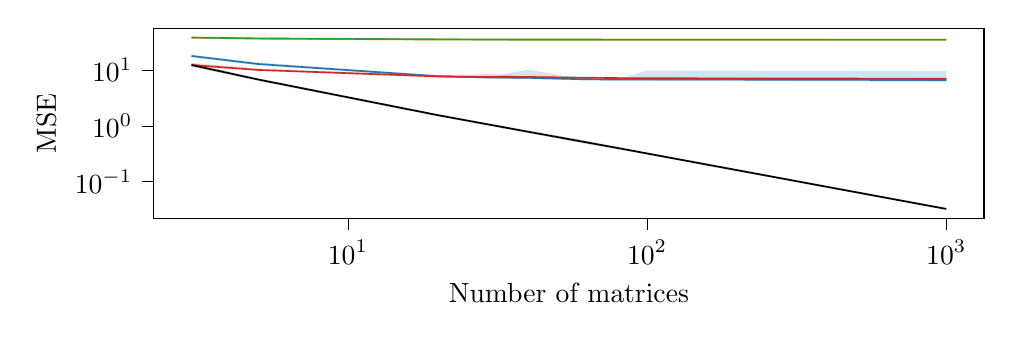
\begin{tikzpicture}

\definecolor{crimson2143940}{RGB}{214,39,40}
\definecolor{darkgray176}{RGB}{176,176,176}
\definecolor{darkorange25512714}{RGB}{255,127,14}
\definecolor{forestgreen4416044}{RGB}{44,160,44}
\definecolor{lightgray204}{RGB}{204,204,204}
\definecolor{steelblue31119180}{RGB}{31,119,180}

\begin{axis}[
width=\columnwidth,
height=4cm,
legend cell align={left},
legend style={
  fill opacity=0.8,
  draw opacity=1,
  text opacity=1,
  at={(0.03,0.03)},
  anchor=south west,
  draw=lightgray204
},
log basis x={10},
log basis y={10},
tick align=outside,
tick pos=left,
x grid style={darkgray176},
xlabel={Number of matrices},
xmin=2.2437647322819, xmax=1337.03857487278,
xmode=log,
xtick style={color=black},
xtick={0.1,1,10,100,1000,10000,100000},
xticklabels={
  \(\displaystyle {10^{-1}}\),
  \(\displaystyle {10^{0}}\),
  \(\displaystyle {10^{1}}\),
  \(\displaystyle {10^{2}}\),
  \(\displaystyle {10^{3}}\),
  \(\displaystyle {10^{4}}\),
  \(\displaystyle {10^{5}}\)
},
y grid style={darkgray176},
ylabel={MSE},
ymin=0.0218043651445638, ymax=56.0024815737763,
ymode=log,
ytick style={color=black},
ytick={0.001,0.01,0.1,1,10,100,1000},
yticklabels={
  \(\displaystyle {10^{-3}}\),
  \(\displaystyle {10^{-2}}\),
  \(\displaystyle {10^{-1}}\),
  \(\displaystyle {10^{0}}\),
  \(\displaystyle {10^{1}}\),
  \(\displaystyle {10^{2}}\),
  \(\displaystyle {10^{3}}\)
}
]
\path [fill=steelblue31119180, fill opacity=0.2]
(axis cs:3,18.8043389613054)
--(axis cs:3,16.8314875609603)
--(axis cs:5,12.1381896526981)
--(axis cs:20,7.40333054447914)
--(axis cs:30,6.99241936580442)
--(axis cs:40,6.84333140532385)
--(axis cs:60,6.5547090007593)
--(axis cs:80,6.44242941841111)
--(axis cs:100,6.42923176293192)
--(axis cs:1000,6.15031714334588)
--(axis cs:1000,9.57269828056928)
--(axis cs:1000,9.57269828056928)
--(axis cs:100,9.77214297162595)
--(axis cs:80,6.84651314814767)
--(axis cs:60,7.03283275125054)
--(axis cs:40,10.1446648799031)
--(axis cs:30,7.5899688263652)
--(axis cs:20,8.04034681130094)
--(axis cs:5,13.6925881202131)
--(axis cs:3,18.8043389613054)
--cycle;

\path [fill=darkorange25512714, fill opacity=0.2]
(axis cs:3,39.005998009636)
--(axis cs:3,36.8707156277165)
--(axis cs:5,35.5865352644737)
--(axis cs:20,34.5473070558395)
--(axis cs:30,34.579891613708)
--(axis cs:40,34.5237197996682)
--(axis cs:60,34.5172640777862)
--(axis cs:80,34.5040367785707)
--(axis cs:100,34.5406761244513)
--(axis cs:1000,34.6100474756888)
--(axis cs:1000,34.7667457265176)
--(axis cs:1000,34.7667457265176)
--(axis cs:100,35.018072659898)
--(axis cs:80,35.0204169989352)
--(axis cs:60,35.1346156589806)
--(axis cs:40,35.3105106802022)
--(axis cs:30,35.4543696924228)
--(axis cs:20,35.6181967536497)
--(axis cs:5,37.4501666134047)
--(axis cs:3,39.005998009636)
--cycle;

\path [fill=forestgreen4416044, fill opacity=0.2]
(axis cs:3,39.1942675122421)
--(axis cs:3,37.2808363913984)
--(axis cs:5,35.7911711661596)
--(axis cs:20,34.8860863353065)
--(axis cs:30,34.8716226124352)
--(axis cs:40,34.7987963431535)
--(axis cs:60,34.7593184055425)
--(axis cs:80,34.7893520398673)
--(axis cs:100,34.7844604342404)
--(axis cs:1000,34.8937987135023)
--(axis cs:1000,35.0518189132013)
--(axis cs:1000,35.0518189132013)
--(axis cs:100,35.2747395820992)
--(axis cs:80,35.280664789503)
--(axis cs:60,35.3843482742359)
--(axis cs:40,35.491153530183)
--(axis cs:30,35.7177289930558)
--(axis cs:20,35.9151745882271)
--(axis cs:5,37.7412903329415)
--(axis cs:3,39.1942675122421)
--cycle;

\path [fill=crimson2143940, fill opacity=0.2]
(axis cs:3,13.4150106353578)
--(axis cs:3,11.6981243465868)
--(axis cs:5,9.61827227403283)
--(axis cs:20,7.36444461877267)
--(axis cs:30,7.14352133961181)
--(axis cs:40,7.00841372147705)
--(axis cs:60,6.94320751913582)
--(axis cs:80,6.91012783163816)
--(axis cs:100,6.74522525628883)
--(axis cs:1000,6.69264725683738)
--(axis cs:1000,6.94221203330159)
--(axis cs:1000,6.94221203330159)
--(axis cs:100,7.30551547212458)
--(axis cs:80,7.36045805216695)
--(axis cs:60,7.29151580346628)
--(axis cs:40,7.60690213210427)
--(axis cs:30,8.48945039975636)
--(axis cs:20,8.00543821354113)
--(axis cs:5,10.6273361853284)
--(axis cs:3,13.4150106353578)
--cycle;

\path [fill=black, fill opacity=0.2]
(axis cs:3,13.2493448302234)
--(axis cs:3,11.4860534270566)
--(axis cs:5,6.42575481512846)
--(axis cs:20,1.47633412090066)
--(axis cs:30,0.984704248724723)
--(axis cs:40,0.745685316007821)
--(axis cs:60,0.495193991616838)
--(axis cs:80,0.37902380712767)
--(axis cs:100,0.304820634372988)
--(axis cs:1000,0.0311550294148225)
--(axis cs:1000,0.0341197901365598)
--(axis cs:1000,0.0341197901365598)
--(axis cs:100,0.335310339716903)
--(axis cs:80,0.418883868889403)
--(axis cs:60,0.564439336906844)
--(axis cs:40,0.825173648165352)
--(axis cs:30,1.09302438447952)
--(axis cs:20,1.6280331731264)
--(axis cs:5,7.12816348512381)
--(axis cs:3,13.2493448302234)
--cycle;

\addplot [semithick, steelblue31119180]
table {%
3 17.8578669661773
5 12.8155686738752
20 7.73639624547268
30 7.34216999141405
40 7.25532560940202
60 6.85056244981613
80 6.72031984059409
100 6.7701088293971
1000 6.60524420674127
};
\addlegendentry{SCM}
\addplot [semithick, darkorange25512714]
table {%
3 37.9287812137695
5 36.510870869585
20 35.1182093437605
30 34.9814035545661
40 34.8926849163795
60 34.8302189752921
80 34.7929360698527
100 34.7916496247899
1000 34.6521177061983
};
\addlegendentry{LW linear}
\addplot [semithick, forestgreen4416044]
table {%
3 38.1727186345762
5 36.786643404877
20 35.3985798037799
30 35.2478541588808
40 35.1524144312998
60 35.0782768971115
80 35.0594873887069
100 35.0314417745551
1000 34.9673991259342
};
\addlegendentry{OAS}
\addplot [semithick, crimson2143940]
table {%
3 12.3112936200546
5 10.0392129332778
20 7.68102260267098
30 7.48727072899839
40 7.50180091565585
60 7.30395299485244
80 7.16727107641064
100 7.12028507303887
1000 6.98447855227814
};
\addlegendentry{LW nonlinear}
\addplot [semithick, black]
table {%
3 12.279626119493
5 6.77618065458479
20 1.55136016011359
30 1.04161989750938
40 0.785323043157254
60 0.528655778789545
80 0.399959956704565
100 0.320227137484716
1000 0.0325302658364751
};
\addlegendentry{RMT}

\legend{};
\end{axis}

\end{tikzpicture}

%     \caption{$p=5$, $n=7$}
%     \label{fig:subfiga}
%   \end{subfigure}
%   \begin{subfigure}{0.4\textwidth}
%     % This file was created with tikzplotlib v0.10.1.
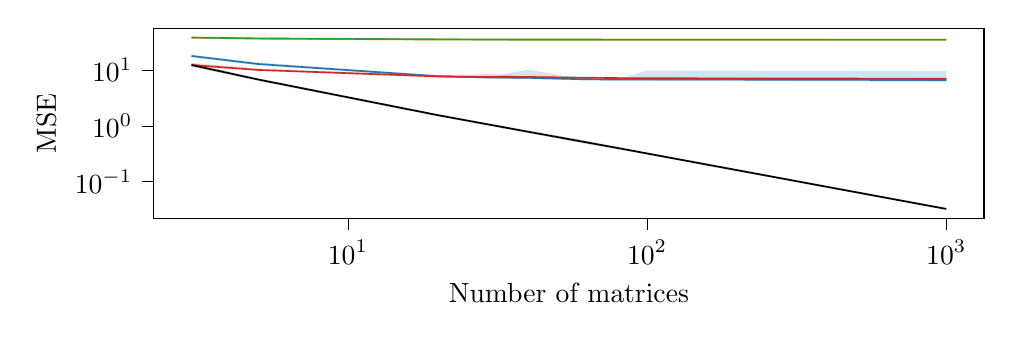
\begin{tikzpicture}

\definecolor{crimson2143940}{RGB}{214,39,40}
\definecolor{darkgray176}{RGB}{176,176,176}
\definecolor{darkorange25512714}{RGB}{255,127,14}
\definecolor{forestgreen4416044}{RGB}{44,160,44}
\definecolor{lightgray204}{RGB}{204,204,204}
\definecolor{steelblue31119180}{RGB}{31,119,180}

\begin{axis}[
width=\columnwidth,
height=4cm,
legend cell align={left},
legend style={
  fill opacity=0.8,
  draw opacity=1,
  text opacity=1,
  at={(0.03,0.03)},
  anchor=south west,
  draw=lightgray204
},
log basis x={10},
log basis y={10},
tick align=outside,
tick pos=left,
x grid style={darkgray176},
xlabel={Number of matrices},
xmin=2.2437647322819, xmax=1337.03857487278,
xmode=log,
xtick style={color=black},
xtick={0.1,1,10,100,1000,10000,100000},
xticklabels={
  \(\displaystyle {10^{-1}}\),
  \(\displaystyle {10^{0}}\),
  \(\displaystyle {10^{1}}\),
  \(\displaystyle {10^{2}}\),
  \(\displaystyle {10^{3}}\),
  \(\displaystyle {10^{4}}\),
  \(\displaystyle {10^{5}}\)
},
y grid style={darkgray176},
ylabel={MSE},
ymin=0.0218043651445638, ymax=56.0024815737763,
ymode=log,
ytick style={color=black},
ytick={0.001,0.01,0.1,1,10,100,1000},
yticklabels={
  \(\displaystyle {10^{-3}}\),
  \(\displaystyle {10^{-2}}\),
  \(\displaystyle {10^{-1}}\),
  \(\displaystyle {10^{0}}\),
  \(\displaystyle {10^{1}}\),
  \(\displaystyle {10^{2}}\),
  \(\displaystyle {10^{3}}\)
}
]
\path [fill=steelblue31119180, fill opacity=0.2]
(axis cs:3,18.8043389613054)
--(axis cs:3,16.8314875609603)
--(axis cs:5,12.1381896526981)
--(axis cs:20,7.40333054447914)
--(axis cs:30,6.99241936580442)
--(axis cs:40,6.84333140532385)
--(axis cs:60,6.5547090007593)
--(axis cs:80,6.44242941841111)
--(axis cs:100,6.42923176293192)
--(axis cs:1000,6.15031714334588)
--(axis cs:1000,9.57269828056928)
--(axis cs:1000,9.57269828056928)
--(axis cs:100,9.77214297162595)
--(axis cs:80,6.84651314814767)
--(axis cs:60,7.03283275125054)
--(axis cs:40,10.1446648799031)
--(axis cs:30,7.5899688263652)
--(axis cs:20,8.04034681130094)
--(axis cs:5,13.6925881202131)
--(axis cs:3,18.8043389613054)
--cycle;

\path [fill=darkorange25512714, fill opacity=0.2]
(axis cs:3,39.005998009636)
--(axis cs:3,36.8707156277165)
--(axis cs:5,35.5865352644737)
--(axis cs:20,34.5473070558395)
--(axis cs:30,34.579891613708)
--(axis cs:40,34.5237197996682)
--(axis cs:60,34.5172640777862)
--(axis cs:80,34.5040367785707)
--(axis cs:100,34.5406761244513)
--(axis cs:1000,34.6100474756888)
--(axis cs:1000,34.7667457265176)
--(axis cs:1000,34.7667457265176)
--(axis cs:100,35.018072659898)
--(axis cs:80,35.0204169989352)
--(axis cs:60,35.1346156589806)
--(axis cs:40,35.3105106802022)
--(axis cs:30,35.4543696924228)
--(axis cs:20,35.6181967536497)
--(axis cs:5,37.4501666134047)
--(axis cs:3,39.005998009636)
--cycle;

\path [fill=forestgreen4416044, fill opacity=0.2]
(axis cs:3,39.1942675122421)
--(axis cs:3,37.2808363913984)
--(axis cs:5,35.7911711661596)
--(axis cs:20,34.8860863353065)
--(axis cs:30,34.8716226124352)
--(axis cs:40,34.7987963431535)
--(axis cs:60,34.7593184055425)
--(axis cs:80,34.7893520398673)
--(axis cs:100,34.7844604342404)
--(axis cs:1000,34.8937987135023)
--(axis cs:1000,35.0518189132013)
--(axis cs:1000,35.0518189132013)
--(axis cs:100,35.2747395820992)
--(axis cs:80,35.280664789503)
--(axis cs:60,35.3843482742359)
--(axis cs:40,35.491153530183)
--(axis cs:30,35.7177289930558)
--(axis cs:20,35.9151745882271)
--(axis cs:5,37.7412903329415)
--(axis cs:3,39.1942675122421)
--cycle;

\path [fill=crimson2143940, fill opacity=0.2]
(axis cs:3,13.4150106353578)
--(axis cs:3,11.6981243465868)
--(axis cs:5,9.61827227403283)
--(axis cs:20,7.36444461877267)
--(axis cs:30,7.14352133961181)
--(axis cs:40,7.00841372147705)
--(axis cs:60,6.94320751913582)
--(axis cs:80,6.91012783163816)
--(axis cs:100,6.74522525628883)
--(axis cs:1000,6.69264725683738)
--(axis cs:1000,6.94221203330159)
--(axis cs:1000,6.94221203330159)
--(axis cs:100,7.30551547212458)
--(axis cs:80,7.36045805216695)
--(axis cs:60,7.29151580346628)
--(axis cs:40,7.60690213210427)
--(axis cs:30,8.48945039975636)
--(axis cs:20,8.00543821354113)
--(axis cs:5,10.6273361853284)
--(axis cs:3,13.4150106353578)
--cycle;

\path [fill=black, fill opacity=0.2]
(axis cs:3,13.2493448302234)
--(axis cs:3,11.4860534270566)
--(axis cs:5,6.42575481512846)
--(axis cs:20,1.47633412090066)
--(axis cs:30,0.984704248724723)
--(axis cs:40,0.745685316007821)
--(axis cs:60,0.495193991616838)
--(axis cs:80,0.37902380712767)
--(axis cs:100,0.304820634372988)
--(axis cs:1000,0.0311550294148225)
--(axis cs:1000,0.0341197901365598)
--(axis cs:1000,0.0341197901365598)
--(axis cs:100,0.335310339716903)
--(axis cs:80,0.418883868889403)
--(axis cs:60,0.564439336906844)
--(axis cs:40,0.825173648165352)
--(axis cs:30,1.09302438447952)
--(axis cs:20,1.6280331731264)
--(axis cs:5,7.12816348512381)
--(axis cs:3,13.2493448302234)
--cycle;

\addplot [semithick, steelblue31119180]
table {%
3 17.8578669661773
5 12.8155686738752
20 7.73639624547268
30 7.34216999141405
40 7.25532560940202
60 6.85056244981613
80 6.72031984059409
100 6.7701088293971
1000 6.60524420674127
};
\addlegendentry{SCM}
\addplot [semithick, darkorange25512714]
table {%
3 37.9287812137695
5 36.510870869585
20 35.1182093437605
30 34.9814035545661
40 34.8926849163795
60 34.8302189752921
80 34.7929360698527
100 34.7916496247899
1000 34.6521177061983
};
\addlegendentry{LW linear}
\addplot [semithick, forestgreen4416044]
table {%
3 38.1727186345762
5 36.786643404877
20 35.3985798037799
30 35.2478541588808
40 35.1524144312998
60 35.0782768971115
80 35.0594873887069
100 35.0314417745551
1000 34.9673991259342
};
\addlegendentry{OAS}
\addplot [semithick, crimson2143940]
table {%
3 12.3112936200546
5 10.0392129332778
20 7.68102260267098
30 7.48727072899839
40 7.50180091565585
60 7.30395299485244
80 7.16727107641064
100 7.12028507303887
1000 6.98447855227814
};
\addlegendentry{LW nonlinear}
\addplot [semithick, black]
table {%
3 12.279626119493
5 6.77618065458479
20 1.55136016011359
30 1.04161989750938
40 0.785323043157254
60 0.528655778789545
80 0.399959956704565
100 0.320227137484716
1000 0.0325302658364751
};
\addlegendentry{RMT}

\legend{};
\end{axis}

\end{tikzpicture}

%     \caption{$p=5$, $n=25$}
%     \label{fig:subfigb}
%   \end{subfigure}
%   \begin{subfigure}{0.4\textwidth}
%     % This file was created with tikzplotlib v0.10.1.
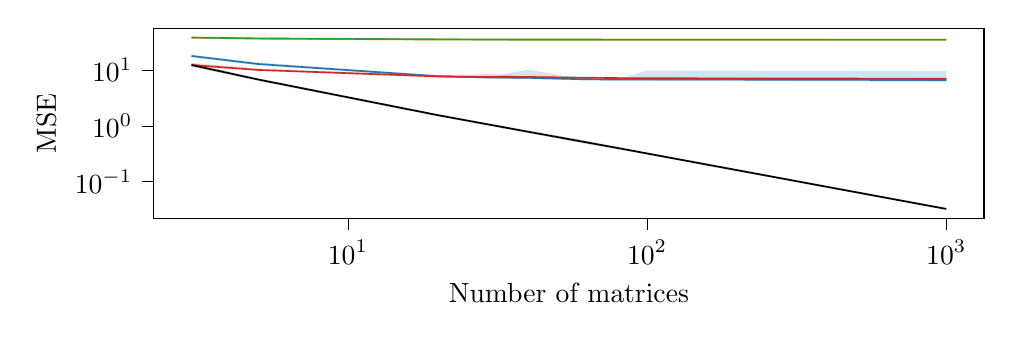
\begin{tikzpicture}

\definecolor{crimson2143940}{RGB}{214,39,40}
\definecolor{darkgray176}{RGB}{176,176,176}
\definecolor{darkorange25512714}{RGB}{255,127,14}
\definecolor{forestgreen4416044}{RGB}{44,160,44}
\definecolor{lightgray204}{RGB}{204,204,204}
\definecolor{steelblue31119180}{RGB}{31,119,180}

\begin{axis}[
width=\columnwidth,
height=4cm,
legend cell align={left},
legend style={
  fill opacity=0.8,
  draw opacity=1,
  text opacity=1,
  at={(0.03,0.03)},
  anchor=south west,
  draw=lightgray204
},
log basis x={10},
log basis y={10},
tick align=outside,
tick pos=left,
x grid style={darkgray176},
xlabel={Number of matrices},
xmin=2.2437647322819, xmax=1337.03857487278,
xmode=log,
xtick style={color=black},
xtick={0.1,1,10,100,1000,10000,100000},
xticklabels={
  \(\displaystyle {10^{-1}}\),
  \(\displaystyle {10^{0}}\),
  \(\displaystyle {10^{1}}\),
  \(\displaystyle {10^{2}}\),
  \(\displaystyle {10^{3}}\),
  \(\displaystyle {10^{4}}\),
  \(\displaystyle {10^{5}}\)
},
y grid style={darkgray176},
ylabel={MSE},
ymin=0.0218043651445638, ymax=56.0024815737763,
ymode=log,
ytick style={color=black},
ytick={0.001,0.01,0.1,1,10,100,1000},
yticklabels={
  \(\displaystyle {10^{-3}}\),
  \(\displaystyle {10^{-2}}\),
  \(\displaystyle {10^{-1}}\),
  \(\displaystyle {10^{0}}\),
  \(\displaystyle {10^{1}}\),
  \(\displaystyle {10^{2}}\),
  \(\displaystyle {10^{3}}\)
}
]
\path [fill=steelblue31119180, fill opacity=0.2]
(axis cs:3,18.8043389613054)
--(axis cs:3,16.8314875609603)
--(axis cs:5,12.1381896526981)
--(axis cs:20,7.40333054447914)
--(axis cs:30,6.99241936580442)
--(axis cs:40,6.84333140532385)
--(axis cs:60,6.5547090007593)
--(axis cs:80,6.44242941841111)
--(axis cs:100,6.42923176293192)
--(axis cs:1000,6.15031714334588)
--(axis cs:1000,9.57269828056928)
--(axis cs:1000,9.57269828056928)
--(axis cs:100,9.77214297162595)
--(axis cs:80,6.84651314814767)
--(axis cs:60,7.03283275125054)
--(axis cs:40,10.1446648799031)
--(axis cs:30,7.5899688263652)
--(axis cs:20,8.04034681130094)
--(axis cs:5,13.6925881202131)
--(axis cs:3,18.8043389613054)
--cycle;

\path [fill=darkorange25512714, fill opacity=0.2]
(axis cs:3,39.005998009636)
--(axis cs:3,36.8707156277165)
--(axis cs:5,35.5865352644737)
--(axis cs:20,34.5473070558395)
--(axis cs:30,34.579891613708)
--(axis cs:40,34.5237197996682)
--(axis cs:60,34.5172640777862)
--(axis cs:80,34.5040367785707)
--(axis cs:100,34.5406761244513)
--(axis cs:1000,34.6100474756888)
--(axis cs:1000,34.7667457265176)
--(axis cs:1000,34.7667457265176)
--(axis cs:100,35.018072659898)
--(axis cs:80,35.0204169989352)
--(axis cs:60,35.1346156589806)
--(axis cs:40,35.3105106802022)
--(axis cs:30,35.4543696924228)
--(axis cs:20,35.6181967536497)
--(axis cs:5,37.4501666134047)
--(axis cs:3,39.005998009636)
--cycle;

\path [fill=forestgreen4416044, fill opacity=0.2]
(axis cs:3,39.1942675122421)
--(axis cs:3,37.2808363913984)
--(axis cs:5,35.7911711661596)
--(axis cs:20,34.8860863353065)
--(axis cs:30,34.8716226124352)
--(axis cs:40,34.7987963431535)
--(axis cs:60,34.7593184055425)
--(axis cs:80,34.7893520398673)
--(axis cs:100,34.7844604342404)
--(axis cs:1000,34.8937987135023)
--(axis cs:1000,35.0518189132013)
--(axis cs:1000,35.0518189132013)
--(axis cs:100,35.2747395820992)
--(axis cs:80,35.280664789503)
--(axis cs:60,35.3843482742359)
--(axis cs:40,35.491153530183)
--(axis cs:30,35.7177289930558)
--(axis cs:20,35.9151745882271)
--(axis cs:5,37.7412903329415)
--(axis cs:3,39.1942675122421)
--cycle;

\path [fill=crimson2143940, fill opacity=0.2]
(axis cs:3,13.4150106353578)
--(axis cs:3,11.6981243465868)
--(axis cs:5,9.61827227403283)
--(axis cs:20,7.36444461877267)
--(axis cs:30,7.14352133961181)
--(axis cs:40,7.00841372147705)
--(axis cs:60,6.94320751913582)
--(axis cs:80,6.91012783163816)
--(axis cs:100,6.74522525628883)
--(axis cs:1000,6.69264725683738)
--(axis cs:1000,6.94221203330159)
--(axis cs:1000,6.94221203330159)
--(axis cs:100,7.30551547212458)
--(axis cs:80,7.36045805216695)
--(axis cs:60,7.29151580346628)
--(axis cs:40,7.60690213210427)
--(axis cs:30,8.48945039975636)
--(axis cs:20,8.00543821354113)
--(axis cs:5,10.6273361853284)
--(axis cs:3,13.4150106353578)
--cycle;

\path [fill=black, fill opacity=0.2]
(axis cs:3,13.2493448302234)
--(axis cs:3,11.4860534270566)
--(axis cs:5,6.42575481512846)
--(axis cs:20,1.47633412090066)
--(axis cs:30,0.984704248724723)
--(axis cs:40,0.745685316007821)
--(axis cs:60,0.495193991616838)
--(axis cs:80,0.37902380712767)
--(axis cs:100,0.304820634372988)
--(axis cs:1000,0.0311550294148225)
--(axis cs:1000,0.0341197901365598)
--(axis cs:1000,0.0341197901365598)
--(axis cs:100,0.335310339716903)
--(axis cs:80,0.418883868889403)
--(axis cs:60,0.564439336906844)
--(axis cs:40,0.825173648165352)
--(axis cs:30,1.09302438447952)
--(axis cs:20,1.6280331731264)
--(axis cs:5,7.12816348512381)
--(axis cs:3,13.2493448302234)
--cycle;

\addplot [semithick, steelblue31119180]
table {%
3 17.8578669661773
5 12.8155686738752
20 7.73639624547268
30 7.34216999141405
40 7.25532560940202
60 6.85056244981613
80 6.72031984059409
100 6.7701088293971
1000 6.60524420674127
};
\addlegendentry{SCM}
\addplot [semithick, darkorange25512714]
table {%
3 37.9287812137695
5 36.510870869585
20 35.1182093437605
30 34.9814035545661
40 34.8926849163795
60 34.8302189752921
80 34.7929360698527
100 34.7916496247899
1000 34.6521177061983
};
\addlegendentry{LW linear}
\addplot [semithick, forestgreen4416044]
table {%
3 38.1727186345762
5 36.786643404877
20 35.3985798037799
30 35.2478541588808
40 35.1524144312998
60 35.0782768971115
80 35.0594873887069
100 35.0314417745551
1000 34.9673991259342
};
\addlegendentry{OAS}
\addplot [semithick, crimson2143940]
table {%
3 12.3112936200546
5 10.0392129332778
20 7.68102260267098
30 7.48727072899839
40 7.50180091565585
60 7.30395299485244
80 7.16727107641064
100 7.12028507303887
1000 6.98447855227814
};
\addlegendentry{LW nonlinear}
\addplot [semithick, black]
table {%
3 12.279626119493
5 6.77618065458479
20 1.55136016011359
30 1.04161989750938
40 0.785323043157254
60 0.528655778789545
80 0.399959956704565
100 0.320227137484716
1000 0.0325302658364751
};
\addlegendentry{RMT}

\legend{};
\end{axis}

\end{tikzpicture}

%     \caption{$p=64$, $n=66$}
%     \label{fig:subfiga}
%   \end{subfigure}
%   \begin{subfigure}{0.4\textwidth}
%     % This file was created with tikzplotlib v0.10.1.
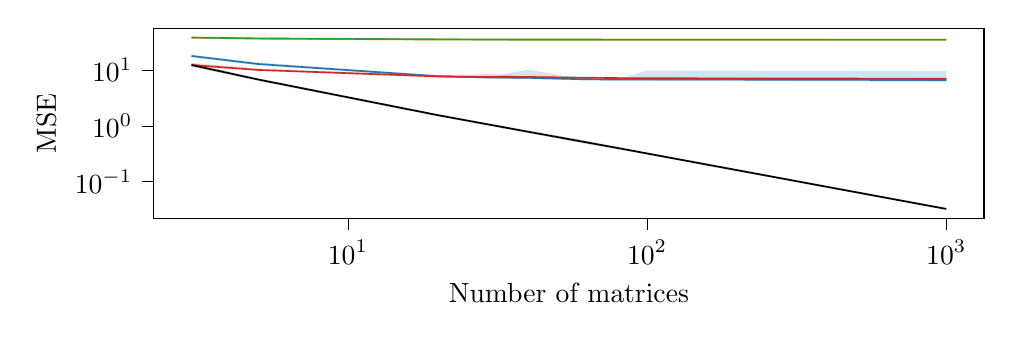
\begin{tikzpicture}

\definecolor{crimson2143940}{RGB}{214,39,40}
\definecolor{darkgray176}{RGB}{176,176,176}
\definecolor{darkorange25512714}{RGB}{255,127,14}
\definecolor{forestgreen4416044}{RGB}{44,160,44}
\definecolor{lightgray204}{RGB}{204,204,204}
\definecolor{steelblue31119180}{RGB}{31,119,180}

\begin{axis}[
width=\columnwidth,
height=4cm,
legend cell align={left},
legend style={
  fill opacity=0.8,
  draw opacity=1,
  text opacity=1,
  at={(0.03,0.03)},
  anchor=south west,
  draw=lightgray204
},
log basis x={10},
log basis y={10},
tick align=outside,
tick pos=left,
x grid style={darkgray176},
xlabel={Number of matrices},
xmin=2.2437647322819, xmax=1337.03857487278,
xmode=log,
xtick style={color=black},
xtick={0.1,1,10,100,1000,10000,100000},
xticklabels={
  \(\displaystyle {10^{-1}}\),
  \(\displaystyle {10^{0}}\),
  \(\displaystyle {10^{1}}\),
  \(\displaystyle {10^{2}}\),
  \(\displaystyle {10^{3}}\),
  \(\displaystyle {10^{4}}\),
  \(\displaystyle {10^{5}}\)
},
y grid style={darkgray176},
ylabel={MSE},
ymin=0.0218043651445638, ymax=56.0024815737763,
ymode=log,
ytick style={color=black},
ytick={0.001,0.01,0.1,1,10,100,1000},
yticklabels={
  \(\displaystyle {10^{-3}}\),
  \(\displaystyle {10^{-2}}\),
  \(\displaystyle {10^{-1}}\),
  \(\displaystyle {10^{0}}\),
  \(\displaystyle {10^{1}}\),
  \(\displaystyle {10^{2}}\),
  \(\displaystyle {10^{3}}\)
}
]
\path [fill=steelblue31119180, fill opacity=0.2]
(axis cs:3,18.8043389613054)
--(axis cs:3,16.8314875609603)
--(axis cs:5,12.1381896526981)
--(axis cs:20,7.40333054447914)
--(axis cs:30,6.99241936580442)
--(axis cs:40,6.84333140532385)
--(axis cs:60,6.5547090007593)
--(axis cs:80,6.44242941841111)
--(axis cs:100,6.42923176293192)
--(axis cs:1000,6.15031714334588)
--(axis cs:1000,9.57269828056928)
--(axis cs:1000,9.57269828056928)
--(axis cs:100,9.77214297162595)
--(axis cs:80,6.84651314814767)
--(axis cs:60,7.03283275125054)
--(axis cs:40,10.1446648799031)
--(axis cs:30,7.5899688263652)
--(axis cs:20,8.04034681130094)
--(axis cs:5,13.6925881202131)
--(axis cs:3,18.8043389613054)
--cycle;

\path [fill=darkorange25512714, fill opacity=0.2]
(axis cs:3,39.005998009636)
--(axis cs:3,36.8707156277165)
--(axis cs:5,35.5865352644737)
--(axis cs:20,34.5473070558395)
--(axis cs:30,34.579891613708)
--(axis cs:40,34.5237197996682)
--(axis cs:60,34.5172640777862)
--(axis cs:80,34.5040367785707)
--(axis cs:100,34.5406761244513)
--(axis cs:1000,34.6100474756888)
--(axis cs:1000,34.7667457265176)
--(axis cs:1000,34.7667457265176)
--(axis cs:100,35.018072659898)
--(axis cs:80,35.0204169989352)
--(axis cs:60,35.1346156589806)
--(axis cs:40,35.3105106802022)
--(axis cs:30,35.4543696924228)
--(axis cs:20,35.6181967536497)
--(axis cs:5,37.4501666134047)
--(axis cs:3,39.005998009636)
--cycle;

\path [fill=forestgreen4416044, fill opacity=0.2]
(axis cs:3,39.1942675122421)
--(axis cs:3,37.2808363913984)
--(axis cs:5,35.7911711661596)
--(axis cs:20,34.8860863353065)
--(axis cs:30,34.8716226124352)
--(axis cs:40,34.7987963431535)
--(axis cs:60,34.7593184055425)
--(axis cs:80,34.7893520398673)
--(axis cs:100,34.7844604342404)
--(axis cs:1000,34.8937987135023)
--(axis cs:1000,35.0518189132013)
--(axis cs:1000,35.0518189132013)
--(axis cs:100,35.2747395820992)
--(axis cs:80,35.280664789503)
--(axis cs:60,35.3843482742359)
--(axis cs:40,35.491153530183)
--(axis cs:30,35.7177289930558)
--(axis cs:20,35.9151745882271)
--(axis cs:5,37.7412903329415)
--(axis cs:3,39.1942675122421)
--cycle;

\path [fill=crimson2143940, fill opacity=0.2]
(axis cs:3,13.4150106353578)
--(axis cs:3,11.6981243465868)
--(axis cs:5,9.61827227403283)
--(axis cs:20,7.36444461877267)
--(axis cs:30,7.14352133961181)
--(axis cs:40,7.00841372147705)
--(axis cs:60,6.94320751913582)
--(axis cs:80,6.91012783163816)
--(axis cs:100,6.74522525628883)
--(axis cs:1000,6.69264725683738)
--(axis cs:1000,6.94221203330159)
--(axis cs:1000,6.94221203330159)
--(axis cs:100,7.30551547212458)
--(axis cs:80,7.36045805216695)
--(axis cs:60,7.29151580346628)
--(axis cs:40,7.60690213210427)
--(axis cs:30,8.48945039975636)
--(axis cs:20,8.00543821354113)
--(axis cs:5,10.6273361853284)
--(axis cs:3,13.4150106353578)
--cycle;

\path [fill=black, fill opacity=0.2]
(axis cs:3,13.2493448302234)
--(axis cs:3,11.4860534270566)
--(axis cs:5,6.42575481512846)
--(axis cs:20,1.47633412090066)
--(axis cs:30,0.984704248724723)
--(axis cs:40,0.745685316007821)
--(axis cs:60,0.495193991616838)
--(axis cs:80,0.37902380712767)
--(axis cs:100,0.304820634372988)
--(axis cs:1000,0.0311550294148225)
--(axis cs:1000,0.0341197901365598)
--(axis cs:1000,0.0341197901365598)
--(axis cs:100,0.335310339716903)
--(axis cs:80,0.418883868889403)
--(axis cs:60,0.564439336906844)
--(axis cs:40,0.825173648165352)
--(axis cs:30,1.09302438447952)
--(axis cs:20,1.6280331731264)
--(axis cs:5,7.12816348512381)
--(axis cs:3,13.2493448302234)
--cycle;

\addplot [semithick, steelblue31119180]
table {%
3 17.8578669661773
5 12.8155686738752
20 7.73639624547268
30 7.34216999141405
40 7.25532560940202
60 6.85056244981613
80 6.72031984059409
100 6.7701088293971
1000 6.60524420674127
};
\addlegendentry{SCM}
\addplot [semithick, darkorange25512714]
table {%
3 37.9287812137695
5 36.510870869585
20 35.1182093437605
30 34.9814035545661
40 34.8926849163795
60 34.8302189752921
80 34.7929360698527
100 34.7916496247899
1000 34.6521177061983
};
\addlegendentry{LW linear}
\addplot [semithick, forestgreen4416044]
table {%
3 38.1727186345762
5 36.786643404877
20 35.3985798037799
30 35.2478541588808
40 35.1524144312998
60 35.0782768971115
80 35.0594873887069
100 35.0314417745551
1000 34.9673991259342
};
\addlegendentry{OAS}
\addplot [semithick, crimson2143940]
table {%
3 12.3112936200546
5 10.0392129332778
20 7.68102260267098
30 7.48727072899839
40 7.50180091565585
60 7.30395299485244
80 7.16727107641064
100 7.12028507303887
1000 6.98447855227814
};
\addlegendentry{LW nonlinear}
\addplot [semithick, black]
table {%
3 12.279626119493
5 6.77618065458479
20 1.55136016011359
30 1.04161989750938
40 0.785323043157254
60 0.528655778789545
80 0.399959956704565
100 0.320227137484716
1000 0.0325302658364751
};
\addlegendentry{RMT}

\legend{};
\end{axis}

\end{tikzpicture}

%     \caption{$p=64$, $n=128$}
%     \label{fig:subfigb}
%   \end{subfigure}
%   \begin{subfigure}{0.4\textwidth}
%     % This file was created with tikzplotlib v0.10.1.
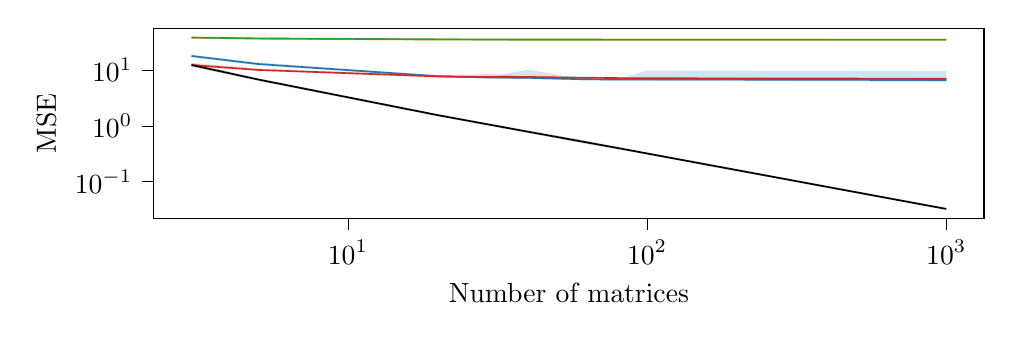
\begin{tikzpicture}

\definecolor{crimson2143940}{RGB}{214,39,40}
\definecolor{darkgray176}{RGB}{176,176,176}
\definecolor{darkorange25512714}{RGB}{255,127,14}
\definecolor{forestgreen4416044}{RGB}{44,160,44}
\definecolor{lightgray204}{RGB}{204,204,204}
\definecolor{steelblue31119180}{RGB}{31,119,180}

\begin{axis}[
width=\columnwidth,
height=4cm,
legend cell align={left},
legend style={
  fill opacity=0.8,
  draw opacity=1,
  text opacity=1,
  at={(0.03,0.03)},
  anchor=south west,
  draw=lightgray204
},
log basis x={10},
log basis y={10},
tick align=outside,
tick pos=left,
x grid style={darkgray176},
xlabel={Number of matrices},
xmin=2.2437647322819, xmax=1337.03857487278,
xmode=log,
xtick style={color=black},
xtick={0.1,1,10,100,1000,10000,100000},
xticklabels={
  \(\displaystyle {10^{-1}}\),
  \(\displaystyle {10^{0}}\),
  \(\displaystyle {10^{1}}\),
  \(\displaystyle {10^{2}}\),
  \(\displaystyle {10^{3}}\),
  \(\displaystyle {10^{4}}\),
  \(\displaystyle {10^{5}}\)
},
y grid style={darkgray176},
ylabel={MSE},
ymin=0.0218043651445638, ymax=56.0024815737763,
ymode=log,
ytick style={color=black},
ytick={0.001,0.01,0.1,1,10,100,1000},
yticklabels={
  \(\displaystyle {10^{-3}}\),
  \(\displaystyle {10^{-2}}\),
  \(\displaystyle {10^{-1}}\),
  \(\displaystyle {10^{0}}\),
  \(\displaystyle {10^{1}}\),
  \(\displaystyle {10^{2}}\),
  \(\displaystyle {10^{3}}\)
}
]
\path [fill=steelblue31119180, fill opacity=0.2]
(axis cs:3,18.8043389613054)
--(axis cs:3,16.8314875609603)
--(axis cs:5,12.1381896526981)
--(axis cs:20,7.40333054447914)
--(axis cs:30,6.99241936580442)
--(axis cs:40,6.84333140532385)
--(axis cs:60,6.5547090007593)
--(axis cs:80,6.44242941841111)
--(axis cs:100,6.42923176293192)
--(axis cs:1000,6.15031714334588)
--(axis cs:1000,9.57269828056928)
--(axis cs:1000,9.57269828056928)
--(axis cs:100,9.77214297162595)
--(axis cs:80,6.84651314814767)
--(axis cs:60,7.03283275125054)
--(axis cs:40,10.1446648799031)
--(axis cs:30,7.5899688263652)
--(axis cs:20,8.04034681130094)
--(axis cs:5,13.6925881202131)
--(axis cs:3,18.8043389613054)
--cycle;

\path [fill=darkorange25512714, fill opacity=0.2]
(axis cs:3,39.005998009636)
--(axis cs:3,36.8707156277165)
--(axis cs:5,35.5865352644737)
--(axis cs:20,34.5473070558395)
--(axis cs:30,34.579891613708)
--(axis cs:40,34.5237197996682)
--(axis cs:60,34.5172640777862)
--(axis cs:80,34.5040367785707)
--(axis cs:100,34.5406761244513)
--(axis cs:1000,34.6100474756888)
--(axis cs:1000,34.7667457265176)
--(axis cs:1000,34.7667457265176)
--(axis cs:100,35.018072659898)
--(axis cs:80,35.0204169989352)
--(axis cs:60,35.1346156589806)
--(axis cs:40,35.3105106802022)
--(axis cs:30,35.4543696924228)
--(axis cs:20,35.6181967536497)
--(axis cs:5,37.4501666134047)
--(axis cs:3,39.005998009636)
--cycle;

\path [fill=forestgreen4416044, fill opacity=0.2]
(axis cs:3,39.1942675122421)
--(axis cs:3,37.2808363913984)
--(axis cs:5,35.7911711661596)
--(axis cs:20,34.8860863353065)
--(axis cs:30,34.8716226124352)
--(axis cs:40,34.7987963431535)
--(axis cs:60,34.7593184055425)
--(axis cs:80,34.7893520398673)
--(axis cs:100,34.7844604342404)
--(axis cs:1000,34.8937987135023)
--(axis cs:1000,35.0518189132013)
--(axis cs:1000,35.0518189132013)
--(axis cs:100,35.2747395820992)
--(axis cs:80,35.280664789503)
--(axis cs:60,35.3843482742359)
--(axis cs:40,35.491153530183)
--(axis cs:30,35.7177289930558)
--(axis cs:20,35.9151745882271)
--(axis cs:5,37.7412903329415)
--(axis cs:3,39.1942675122421)
--cycle;

\path [fill=crimson2143940, fill opacity=0.2]
(axis cs:3,13.4150106353578)
--(axis cs:3,11.6981243465868)
--(axis cs:5,9.61827227403283)
--(axis cs:20,7.36444461877267)
--(axis cs:30,7.14352133961181)
--(axis cs:40,7.00841372147705)
--(axis cs:60,6.94320751913582)
--(axis cs:80,6.91012783163816)
--(axis cs:100,6.74522525628883)
--(axis cs:1000,6.69264725683738)
--(axis cs:1000,6.94221203330159)
--(axis cs:1000,6.94221203330159)
--(axis cs:100,7.30551547212458)
--(axis cs:80,7.36045805216695)
--(axis cs:60,7.29151580346628)
--(axis cs:40,7.60690213210427)
--(axis cs:30,8.48945039975636)
--(axis cs:20,8.00543821354113)
--(axis cs:5,10.6273361853284)
--(axis cs:3,13.4150106353578)
--cycle;

\path [fill=black, fill opacity=0.2]
(axis cs:3,13.2493448302234)
--(axis cs:3,11.4860534270566)
--(axis cs:5,6.42575481512846)
--(axis cs:20,1.47633412090066)
--(axis cs:30,0.984704248724723)
--(axis cs:40,0.745685316007821)
--(axis cs:60,0.495193991616838)
--(axis cs:80,0.37902380712767)
--(axis cs:100,0.304820634372988)
--(axis cs:1000,0.0311550294148225)
--(axis cs:1000,0.0341197901365598)
--(axis cs:1000,0.0341197901365598)
--(axis cs:100,0.335310339716903)
--(axis cs:80,0.418883868889403)
--(axis cs:60,0.564439336906844)
--(axis cs:40,0.825173648165352)
--(axis cs:30,1.09302438447952)
--(axis cs:20,1.6280331731264)
--(axis cs:5,7.12816348512381)
--(axis cs:3,13.2493448302234)
--cycle;

\addplot [semithick, steelblue31119180]
table {%
3 17.8578669661773
5 12.8155686738752
20 7.73639624547268
30 7.34216999141405
40 7.25532560940202
60 6.85056244981613
80 6.72031984059409
100 6.7701088293971
1000 6.60524420674127
};
\addlegendentry{SCM}
\addplot [semithick, darkorange25512714]
table {%
3 37.9287812137695
5 36.510870869585
20 35.1182093437605
30 34.9814035545661
40 34.8926849163795
60 34.8302189752921
80 34.7929360698527
100 34.7916496247899
1000 34.6521177061983
};
\addlegendentry{LW linear}
\addplot [semithick, forestgreen4416044]
table {%
3 38.1727186345762
5 36.786643404877
20 35.3985798037799
30 35.2478541588808
40 35.1524144312998
60 35.0782768971115
80 35.0594873887069
100 35.0314417745551
1000 34.9673991259342
};
\addlegendentry{OAS}
\addplot [semithick, crimson2143940]
table {%
3 12.3112936200546
5 10.0392129332778
20 7.68102260267098
30 7.48727072899839
40 7.50180091565585
60 7.30395299485244
80 7.16727107641064
100 7.12028507303887
1000 6.98447855227814
};
\addlegendentry{LW nonlinear}
\addplot [semithick, black]
table {%
3 12.279626119493
5 6.77618065458479
20 1.55136016011359
30 1.04161989750938
40 0.785323043157254
60 0.528655778789545
80 0.399959956704565
100 0.320227137484716
1000 0.0325302658364751
};
\addlegendentry{RMT}

\legend{};
\end{axis}

\end{tikzpicture}

%     \caption{$p=64$, $n=512$}
%     \label{fig:subfigb}
%   \end{subfigure}
  
%   \caption{MSE of the estimated mean towards true mean for different regimes. For all experiments, the number of maximum iterations of the RMT algorithms is set to $100$ and the stopping criterion is set to $10^{-6}$ and Monte-Carlo has been done over $1000$ trials for $p=5$ and $100$ for $p=64$.}
%   \label{fig:mse nmatrices}
% \end{figure*}

\section{Real data learning experiments}

% \begin{table*}[]
%     \centering
%     \begin{tabular}{||c||c|c|c|c||}
%     \hline
%     \multicolumn{5}{|c|}{PhysionetMI, $p=64$, $K=5$, 23 trials/classes, 109 subjects} \\
%     \hline
%     Paradigm & SCM & LW-SCM & Non Linear LW & RMT-KM \\
%     \hline
%     [1,3], 80Hz & {\bf 0.493} & 0.397 & $\times$ & 0.49 \\
%     \hline
%     \hline
%     \multicolumn{5}{|c|}{Schirrmeister2017, $p=128$, $K=4$, 120 trials/classes, 14 subjects} \\
%     \hline
%     Paradigm     & SCM         & LW-SCM & Non Linear LW & RMT-KM \\
%     \hline
%     [0,5], 100Hz & 0.597       & 0.483 & 0.561          & {\bf 0.603} \\
%     \hline
%     \hline
%     \multicolumn{5}{|c|}{Cho2017, $p=64$, $K=2$, 100 trials/classes, 53 subjects} \\
%     \hline
%     Paradigm & SCM & LW-SCM & Non Linear LW & RMT-KM \\
%     \hline
%     [1,3], 128Hz & 0.615 & 0.609 & 0.601 & {\bf 0.622} \\
%     \hline
%     \hline
%     \multicolumn{5}{|c|}{Lee2019, $p=62$, $K=2$, 100 trials/classes, 55 subjects} \\
%     \hline
%     Paradigm & SCM & LW-SCM & Non Linear LW & RMT-KM \\
%     \hline
%     [2,3], 100Hz & {\bf 0.666} & 0.642 & 0.626 & 0.66 \\
%     \hline
%     \hline
%     \multicolumn{5}{|c|}{Weibo2014, $p=60$, $K=7$, 80 trials/classes, 10 subjects} \\
%     \hline
%     Paradigm & SCM & LW-SCM & Non Linear LW & RMT-KM \\
%     \hline
%     [1,3], 100Hz & {\bf 0.409} & 0.349 & $\times$ & 0.403 \\
%     \hline
%     \hline
%     \multicolumn{5}{|c|}{MunichMI, $p=128$, $K=2$, 150 trials/classes, 10 subjects} \\
%     \hline
%     Paradigm & SCM & LW-SCM & Non Linear LW & RMT-KM \\
%     \hline
%     [0,7], 100Hz & 0.632 & 0.624 & $\times$ & {\bf 0.638} \\
%     \hline
%     \end{tabular}
%     \caption{Classification results for motor imaging data}
%     \label{tab:my_label}
% \end{table*}

\begin{table*}[t]
    \centering
    \begin{tabular}{rcccc}
        & SCM & LW & LW-NL & RMT \\
        \cline{2-5}
        GrosseWentrup09 & 0.632 $\pm$ 0.0867& 0.624 $\pm$ 0.0829 & $\times$ & {\bf 0.638 $\pm$ 0.0917} \\
        Schirmeister17 & 0.597 $\pm$  0.139 & 0.483 $\pm$ 0.0958 & 0.561 $\pm$ 0.120 & {\bf 0.603 $\pm$ 0.120} \\
        Cho17 & 0.615 $\pm$ 0.158 & 0.609 $\pm$ 0.136 & 0.601 $\pm$ 0.131 & {\bf 0.622 $\pm$ 0.158} \\
        Lee19 & {\bf 0.666 $\pm$ 0.138} & 0.642 $\pm$ 0.130 & 0.626 $\pm$ 0.126 & 0.66 $\pm$ 0.137\\
    \end{tabular}
    \caption{Classification results on EEG motor imaging data.}
    \label{tab:eeg_mi}
\end{table*}

\begin{table*}[t]
\centering
\begin{tabular}{rcccccccc}
                              &               &                       & \multicolumn{2}{c}{SCM} & \multicolumn{2}{c}{LW} & \multicolumn{2}{c}{RMT}         \\
                              & $\nfeatures$ & $\nsamples$ & acc             & mIoU  & acc          & mIoU        & acc            & mIoU           \\ \cline{2-9} 
\multirow{4}{*}{Indian pines} & 5             & 5$\times$5            & 0.385           & 0.278 & 0.302        & 0.204       & \textbf{0.454} & \textbf{0.367} \\
                              % & 10            & 5$\times$5            & 0.363           & 0.243 & 0.313        & 0.218       & \textbf{0.422} & \textbf{0.301} \\
                              % & 12            & 7$\times$7            & 0.341           & 0.215 & 0.344        & 0.245       & \textbf{0.446} & \textbf{0.320} \\
                              & 16            & 5$\times$5            & 0.357           & 0.229 & 0.316        & 0.215       & \textbf{0.413} & \textbf{0.284} \\ & 24            & 7$\times$7            & 0.377           & 0.253 & 0.359        & 0.248       & \textbf{0.453} & \textbf{0.285} \\
                              % & 32            & 7$\times$7            & 0.404           & 0.261 & 0.349        & 0.247       & \textbf{0.46} & \textbf{0.288} \\
                              \cline{2-9} 
\multirow{4}{*}{Salinas}      & 5             & 5$\times$5            & 0.542           & 0.382 & 0.402        & 0.252       & \textbf{0.777} & \textbf{0.631} \\
                              & 10            & 7$\times$7            & 0.525           & 0.34  & 0.449        & 0.303       & \textbf{0.746} & \textbf{0.532} \\
                              % & 10            & 9$\times$9            & 0.489           & 0.323 & 0.433        & 0.271       & \textbf{0.603} & \textbf{0.446} \\
                              & 16            & 11$\times$11          & 0.497           & 0.317 & 0.404        & 0.244       & \textbf{0.632} & \textbf{0.461} \\ \cline{2-9} 
% \multirow{2}{*}{PaviaU}       & 5             & 5$\times$5            & \textbf{0.452}  & 0.288 & 0.38         & 0.273       & 0.435          & \textbf{0.463} \\
%                               & 10            & 5$\times$5            & 0.44            & 0.291 & -            & -           & \textbf{0.51}  & \textbf{0.451} \\ \cline{2-9} 
Pavia                         & 5             & 5$\times$5            & 0.629           & 0.378 & 0.615        & 0.319       & \textbf{0.819} & \textbf{0.549} \\ \cline{2-9} 
KSC                           & 5             & 5$\times$5   & 0.263           & 0.167 & 0.247        & 0.169       & \textbf{0.377} & \textbf{0.222}
\end{tabular}
\caption{Clustering results for hyperspectral data. For Indian pines, we did 10 initializations and 5 for the other datasets.}
\label{tab:hyperspectral}
\end{table*}

To assess the practical relevance of the proposed RMT-based mean estimation method, two real-world scenarios are considered:
(\emph{i}) electroencephalography (EEG) classification using Nearest Centroid classifiers and (\emph{ii}) clustering of hyperspectral images using K-Means algorithms.
Various strategies were implemented for mean computation and distance. Specifically, for mean estimation, we consider two step strategies where we first estimate covariances and then compute their generic Fréchet mean associated with~\eqref{eq:Fisher_dist}.
As before, we consider the SCM, linear Ledoit-Wolf (LW) and non-linear Ledoit-Wolf (LW-NL) estimators.
These methods were then benchmarked against our proposed RMT-based Nearest Centroid and K-Means algorithms, as detailed in Section~\ref{sec:mean:learning}. The development and evaluation of these methods were conducted in Python. Specifically, SCM and LW implementations were sourced from the scikit-learn library~\cite{pedregosa2018scikitlearn}, while LW-NL comes from scikit-RMT\footnote{\url{https://scikit-rmt.readthedocs.io/}}. The conventional Fréchet means, standard Nearest Centroid and K-Means algorithms were taken from the pyRiemann library~\cite{alexandre_barachant_2023_8059038}.


\subsection{EEG data}

We initiated our analysis by assessing the Nearest Centroid classifier's efficacy on EEG data, specifically focusing on motor imagery datasets accessible via the MOABB platform~\cite{Aristimunha_Mother_of_all_2023}.
In this context, subjects participate in experiments where they are instructed to mentally simulate various movements, encompassing actions like the motion of the left or right hand, feet, tongue, among others.
The following datasets are used:
GrosseWentrup2009, where $\nclasses=2$, $\nfeatures=128$, signals resampled to $100$Hz;
Schirmeister2017, where  $\nclasses=4$, $\nfeatures=128$, signals resampled to $100$Hz;
Cho2017, where  $\nclasses=2$, $\nfeatures=64$, signals resampled to $128$Hz, trials taken from 1s to 3s;
Lee2019, where  $\nclasses=2$, $\nfeatures=62$, signals resampled to $100$Hz, trials taken from 2s to 3s.



% Results are displayed in Table~\ref{tab:eeg_mi}.
% We observe that SCM and RMT feature similar performance for all datasets, RMT yielding a slight improvement on three of the four.
% In comparison, the accuracies of LW and LW-NL are lower.
% For GrosseWentrup2009, we were even unable to get LW-NL to work as the covariance estimator gave non SPD matrices.
% Hence, RMT is by far the most reliable regularized method on these data.
% However, the small difference with SCM does not make RMT worth the effort for this application.

The outcomes are summarized in Table~\ref{tab:eeg_mi}. An analysis of the results reveals that the SCM and RMT methods demonstrate comparable levels of performance across all datasets, with RMT achieving marginal enhancements in three out of the four datasets. Conversely, the accuracy rates for both LW and LW-NL are notably lower. Specifically, in the case of GrosseWentrup2009, the LW-NL method encountered issues, failing to produce SPD matrices as required, rendering it non-functional. This observation underscores the superior reliability of the RMT method as a regularization technique for these datasets. However, given the minimal performance gap between RMT and SCM, the incremental benefit of RMT may not justify the additional complexity for this particular application.

\subsection{Hyperspectral data}





Our second experiment with real data delves into the clustering of hyperspectral remote sensing datasets, including Indian Pines, Salinas, Pavia, and KSC%
\footnote{
    Available at \url{https://www.ehu.eus/ccwintco/index.php/Hyperspectral_Remote_Sensing_Scenes}.
}.
 These datasets are inherently diverse, characterized by a unique number of bands and classes. They also feature annotated ground truths. Certain zones labeled as "undefined" are considered unreliable and hence are omitted from the accuracy calculations of the clustering methods. Nevertheless, these zones are included during the clustering phase to ensure realistic evaluation. 

 Data preprocessing involves three main steps: normalizing data by subtracting the image's global mean, employing Principal Component Analysis (PCA) to select a set number of channels $\nfeatures$ as per prior research~\cite{9627641}, and using a sliding window with overlap for data sampling around each pixel. We excluded the LW-NL method due to numerical instability. The K-means algorithm, capped at $100$ iterations with early stopping at a $10^{-4}$ tolerance, concludes with a linear assignment optimization to align the clustered image with ground truth, optimizing classification accuracy.
 
% The data preprocessing involves a structured three-step approach. Initially, we normalize the data by subtracting the global mean of the image. Next, we utilize Principal Component Analysis (PCA) to maintain a predetermined number of channels $\nfeatures$. This step is vital as prior research~\cite{9627641} indicates that a limited number of principal components can effectively represent these datasets. Finally, we implement a sliding window technique with overlap to gather data samples around each pixel for clustering. Due to challenges in achieving numerical stability, we exclude the method based on LW-NL from our experiments. The K-means algorithm is configured with a cap of $100$ iterations, complemented by an early stopping mechanism activated by a tolerance threshold of $10^{-4}$. After clustering, we align the segmented image with the ground truth classes by executing a linear assignment optimization, aiming to maximize the classification accuracy.


% Results are reported in Table~\ref{tab:hyperspectral}.
% Computed metrics are the accuracy of classification and the mean intersection over union criterion.
% Our proposed method RMT outperforms both SCM and LW over all datasets for every feature and sample sizes considered.
% We believe that this is can be explained thanks to the fact that the number of matrices per class (one per pixel belonging to the class) in this scenario is very high%
% \footnote{
%     It indeed relates to our simulations: in such a case, our proposed RMT corrected mean is way more accurate than the others.
% }.
% %
% In conclusion, our RMT based approach is extremely advantageous for these data.

% The results are presented in Table~\ref{tab:hyperspectral}, where we assess the performance using two key metrics: the accuracy of classification and the mean intersection over union criterion. The RMT method, as proposed, consistently surpasses both SCM and LW across all datasets, considering various feature and sample sizes. This superior performance can be attributed to the high number of matrices per class in these datasets, where each pixel associated with a class contributes one matrix. Indeed, this finding aligns with our simulation results: in scenarios where the number of matrices per class is substantial, our RMT-corrected mean exhibits significantly higher accuracy compared to alternative methods. Hence, the RMT-based approach proves to be exceptionally beneficial for these types of data, establishing its efficacy in scenarios involving a large number of matrices per class.

The results, detailed in Table~\ref{tab:hyperspectral}, evaluate classification accuracy and mean intersection over union. Our RMT method consistently outperforms SCM and LW across all datasets and varying feature/sample sizes. In our opinion, this success can be attributed to the high number of matrices per class in these datasets, resonating with our simulation insights: in such contexts, the RMT-corrected mean significantly enhances accuracy. In essence, for data scenarios with extensive matrices per class, the RMT approach proves highly effective.

% The study utilizes remote sensing datasets, namely Indian Pines, Salinas, Pavia, and KSC\footnote{Available at \url{https://www.ehu.eus/ccwintco/index.php/Hyperspectral_Remote_Sensing_Scenes}.}. Each dataset comes with a unique number of bands and classes, making the experimentation diverse. The ground truth is deemed unreliable in zones marked as "undefined." Consequently, we exclude these zones from the accuracy computation of clustering methods but they are still used in the clustering step, ensuring a robust evaluation process. Our preprocessing pipeline involves three key steps. First, we remove the global mean of the image to normalize the data. Second, we employ Principal Component Analysis (PCA) to retain a specified number, denoted as $p$, of channels. This step is crucial, as prior studies on these datasets have demonstrated that a few principal directions allow for good representation of the dataset \cite{9627641}. Lastly, we adopt a sliding window approach with overlap to extract data samples in the neighborhood of each pixel to cluster.
% We exclude the LW non-linear method from our experiments due to challenges in achieving numerical stability.  The maximum number of iterations for the K-means algorithm is set to $100$, and early stopping is implemented with a tolerance of $10^{-4}$. Finally, to match the obtained segmented image to the same class numbers of the ground-truth, we solve a linear assignment optimization that maximizes the classification.

% The results over the all the datasets are reported in Table \ref{tab:hyperspectral}. The computed metrics are the accuracy of classification and the mean intersection over union criterion. Interestingly, we observe that our proposed method outperforms both SCM and LW covariance estimation approaches over all the datasets and features size. This can be explained thanks to the fact that the number of matrices per class (one per pixel belonging to the class) in this scenario is very high. As shown in Figure \ref{fig:mse nmatrices}, our method fares the best in the scenarios where the number of matrices is high. These results show that the proposed approach is competitive in real-world applications.



\subsection{Discussion}
The first thing that we notice on these real data learning experiments is the is the lower performance of the methods associated with the linear and non-linear Ledoit-Wolf estimators.
%
For LW, this is in accordance with our simulations.
It is likely that this is because the true covariance matrices are in fact quite far from the identity matrix.
So, linearly shrinking toward the identity does not improve estimation in this case.
%
For LW-NL, this is more surprising.
On these real data, LW-NL has proved itself numerically unstable and unable to consistently provide SPD matrices.

Concerning our RMT-based method, we observe that:
\begin{itemize}
    \item When the number of samples $\nsamples$ is sufficiently big as compared to the dimension $\nfeatures$, our proposed RMT mean becomes equivalent to the usual Fisher mean.
    In this case, one can expect to obtain very similar results with our method as compared to the method associated with the SCM.
    This is indeed what we observe with EEG data, for which a rather large $\nsamples$ is available (and needed to capture the information contained in the data).
    \item When $\nsamples$ is comparable to $\nfeatures$, then our performance depends on the number of matrices $\nmatrices$ available to compute the mean:
    \begin{itemize}
        \item[$\circ$] when $\nmatrices$ is very small, the issue is that there is a clear statistical dependence introduced between the estimated mean and the data at hand.
        In this case, the RMT distance estimator can become irrelevant and our mean is not very satisfying.
        This is the worst case scenario for our method and its main limitation.
        However, in our simulations, a small number of matrices $\nmatrices$ is enough for our method to be competitive.
        %
        \item[$\circ$] when $\nmatrices$ becomes big, this is where our estimator performs very well.
        In fact, on simulated data, our RMT estimator appears to converge to the true mean as $\nmatrices$ grows while other methods do not.
        For the real hyperspectral data that we consider, we are exactly in this scenario and the performance we obtain corresponds to our simulations, \emph{i.e.}, our method performs really well as compared to other methods.
    \end{itemize}
\end{itemize}


\section{Conclusions and perspectives}
\label{sec:conclusion}

% This paper first proposes a new regularized covariance estimate based on an improved distance between two covariances given in \cite{couillet2019random}. Compared with \cite{tiomoko2019random}, this first result for covariance estimation is slightly different, as the problem of independence between the two matrices is better taken into account in the algorithm and a new stopping criterion based on statistical considerations is proposed. Above all, this new result has made it possible to derive the main contribution of the article: a new Fréchet mean algorithm for SPD matrices in a regime of low sample support that is based on a Riemannian gradient on the manifold of SPD matrices. The nearest centroid classifier and the K-means algorithms based on this new barycenter give better results than conventional methods, especially when the number of matrices for each class is high. 

The first part of this paper presents a refined regularized covariance estimator, building upon the corrected squared distance outlined in \cite{couillet2019random}. While this work aligns closely with \cite{tiomoko2019random}, it introduces subtle yet noteworthy enhancements, including a more comprehensive treatment of matrix independence and a new stopping criterion rooted in statistical principles. The primary contribution, however, is the development of a novel Fréchet mean algorithm tailored for random matrices under conditions of low sample support, utilizing a Riemannian gradient on the SPD matrix manifold. When applied to Nearest Centroid classifiers and K-means clustering, this new method demonstrates great potential. It appears very advantageous when dealing with a large number of matrices per class, offering a big improvement over traditional methods in this case.



\section*{Acknowledgement}
This research was supported by DATAIA Convergence Institute as part of the ``Programme d’Investissement d’Avenir", (ANR-17-CONV-0003) operated by Laboratoire des Signaux et Systèmes.


\section*{Impact Statement}
This paper presents work whose goal is to advance the field of Machine Learning. There are many potential societal consequences of our work, none which we feel must be specifically highlighted here.


\bibliographystyle{icml2024}
\bibliography{references.bib}

%%%%%%%%%%%%%%%%%%%%%%%%%%%%%%%%%%%%%%%%%%%%%%%%%%%%%%%%%%%%%%%%%%%%%%%%%%%%%%%
%%%%%%%%%%%%%%%%%%%%%%%%%%%%%%%%%%%%%%%%%%%%%%%%%%%%%%%%%%%%%%%%%%%%%%%%%%%%%%%
% APPENDIX
%%%%%%%%%%%%%%%%%%%%%%%%%%%%%%%%%%%%%%%%%%%%%%%%%%%%%%%%%%%%%%%%%%%%%%%%%%%%%%%
%%%%%%%%%%%%%%%%%%%%%%%%%%%%%%%%%%%%%%%%%%%%%%%%%%%%%%%%%%%%%%%%%%%%%%%%%%%%%%%
\newpage
\appendix
\onecolumn

\section{Proofs of Propositions \ref{prop:Rgrad_eigsfun} and \ref{prop:RMT_Fisher_SCM_deterministic_grad}}
\label{app:proofs}

\subsection{Proof of Proposition \ref{prop:Rgrad_eigsfun}}

\subsection{Proof of Proposition \ref{prop:RMT_Fisher_SCM_deterministic_grad}}


\section{Additional simulations for covariance estimation}
\label{app:simu_RMTCov}



%%%%%%%%%%%%%%%%%%%%%%%%%%%%%%%%%%%%%%%%%%%%%%%%%%%%%%%%%%%%%%%%%%%%%%%%%%%%%%%
%%%%%%%%%%%%%%%%%%%%%%%%%%%%%%%%%%%%%%%%%%%%%%%%%%%%%%%%%%%%%%%%%%%%%%%%%%%%%%%


\end{document}

